% =====================================================================
% Informe técnico final (Fase 4) - Proyecto Integrador de Ciencia de Datos e IA
% Maestría en Inteligencia Artificial - Universidad de La Salle (Bogotá)
% Compilar: pdflatex main && bibtex main && pdflatex main && pdflatex main
%           (o simplemente: latexmk -pdf main.tex)
% =====================================================================
\documentclass[conference,a4paper]{IEEEtran}
\IEEEoverridecommandlockouts

\usepackage[utf8]{inputenc}
\usepackage[T1]{fontenc}
\usepackage[spanish,es-tabla,es-nodecimaldot,es-noshorthands]{babel}
\usepackage{amsmath,amssymb}
\usepackage{graphicx}
\usepackage{booktabs}
\usepackage{multirow}
\usepackage{tabularx}
\usepackage{array}
\usepackage[table]{xcolor}
\usepackage{listings}
\usepackage{cite}
\usepackage{url}
\usepackage[hidelinks]{hyperref}

\definecolor{azul}{HTML}{184F95}
\definecolor{gris}{HTML}{F3F4F5}
\lstset{captionpos=t, abovecaptionskip=4pt, belowcaptionskip=6pt, basicstyle=\ttfamily\scriptsize, backgroundcolor=\color{gris}, frame=single, rulecolor=\color{gray!40},
        keywordstyle=\color{azul}\bfseries, commentstyle=\color{gray}\itshape, columns=fullflexible, breaklines=true,
        language=Python, showstringspaces=false, inputencoding=utf8, extendedchars=true,
        literate={á}{{\'a}}1 {é}{{\'e}}1 {í}{{\'i}}1 {ó}{{\'o}}1 {ú}{{\'u}}1 {ñ}{{\~n}}1 {×}{{$\times$}}1 {→}{{$\rightarrow$}}1}
\renewcommand{\lstlistingname}{Listado}
\renewcommand{\abstractname}{Resumen}
\renewcommand{\IEEEkeywordsname}{Palabras clave}
\newcommand{\coma}{{,}}

\begin{document}

\title{Predicción de diabetes y segmentación de perfiles de riesgo mediante aprendizaje supervisado y no supervisado: un estudio sobre la encuesta BRFSS~2023}

\author{\IEEEauthorblockN{Alain Alexander Camacho Prado}
\IEEEauthorblockA{Maestría en Inteligencia Artificial, Facultad de Ingeniería\\
Universidad de La Salle, Bogotá, Colombia\\
Proyecto Integrador de Ciencia de Datos e IA -- Fase 4 (informe técnico final)}}

\maketitle

\begin{abstract}
Se presenta una solución completa de ciencia de datos para el riesgo de diabetes construida sobre 272.769 registros y 17 predictores autorreportados de la encuesta Behavioral Risk Factor Surveillance System (BRFSS) 2023. El flujo incluye el tratamiento justificado de datos faltantes (simulación MCAR/MAR/MNAR) y atípicos, cuatro variables derivadas, un preprocesamiento encapsulado en \textit{pipelines} que elimina la fuga de datos, una partición estratificada 70/15/15 y el manejo del desbalance (1:5,84) con pesos de clase. Se compararon regresión logística, Random Forest, XGBoost y un perceptrón multicapa en PyTorch; regresiones Ridge, Lasso y ElasticNet y ensambles para el índice de masa corporal (IMC), y K-Means, DBSCAN y el método jerárquico de Ward para la segmentación. Los hiperparámetros se optimizaron con búsqueda aleatoria y validación cruzada estratificada; la incertidumbre se estimó por \textit{bootstrap} y las predicciones se explicaron con TreeSHAP. En el conjunto de prueba, XGBoost alcanzó un AUC-ROC de 0,816 (IC~95\,\%: 0,810--0,821) y un AUC-PR de 0,413, con una sensibilidad de 78,7\,\% al umbral de 0,5; cuatro familias de modelos convergieron en el mismo desempeño, lo que indica un techo impuesto por la información y no por el algoritmo. El R$^2$ del IMC fue de 0,186 y K-Means identificó tres perfiles con prevalencias de diabetes de 3,7\,\%, 22,1\,\% y 27,7\,\%. La solución se desplegó como una aplicación web interactiva en Streamlit, con filtros dinámicos, indicadores clave, predicción en vivo con explicación SHAP y segmentación en el espacio PCA (\url{https://alainkapra-diabetes-brfss2023.streamlit.app}), sobre un repositorio público reproducible (\url{https://github.com/alainkapra/proyecto-diabetes-brfss2023}).
\end{abstract}

\begin{IEEEkeywords}
aprendizaje automático, diabetes, XGBoost, PyTorch, SHAP, K-Means, fuga de datos, clases desbalanceadas, Streamlit, BRFSS.
\end{IEEEkeywords}

% =====================================================================
\section{Introducción}
% =====================================================================
La diabetes mellitus afecta a cerca de 537 millones de adultos en el mundo y una fracción importante desconoce su condición \cite{idf2021}. Las guías recomiendan tamizar con glucosa en ayunas o hemoglobina glicosilada a los adultos con factores de riesgo \cite{ada2024}, y el problema práctico es decidir a quién tamizar con recursos limitados. Las encuestas poblacionales como la BRFSS de los Centros para el Control y la Prevención de Enfermedades (CDC) \cite{cdc2023} permiten construir modelos de riesgo a bajo costo \cite{xie2019}.

Desde la ciencia de datos, el problema reúne cuatro retos que estructuran este trabajo: (i) el \textbf{desbalance de clases}, que vuelve engañosa la exactitud \cite{he2009}; (ii) la \textbf{fuga de datos}, una de las principales causas de resultados irreproducibles en aprendizaje automático \cite{kapoor2023,kaufman2012}; (iii) la \textbf{interpretabilidad}, indispensable cuando el modelo informa decisiones de salud \cite{lundberg2020}, y (iv) el \textbf{despliegue} reproducible del modelo en una herramienta utilizable.

El trabajo se desarrolló en cuatro fases: análisis exploratorio (Fase~1); limpieza, ingeniería de variables y modelo base (Fase~2); modelado avanzado, segmentación, optimización e interpretabilidad (Fase~3), y aplicación web desplegada con repositorio reproducible (Fase~4). Las contribuciones son:
\begin{itemize}
\item Un flujo de preprocesamiento sin fuga, implementado como \texttt{Pipeline} de scikit-learn y compartido entre entrenamiento y aplicación.
\item Una comparación controlada de cuatro familias de clasificadores y seis regresores, con validación cruzada, \textit{bootstrap} pareado y un conjunto de prueba usado una sola vez.
\item Una segmentación validada con tres algoritmos y con una variable externa no usada en el agrupamiento.
\item Explicaciones globales y locales con SHAP, y una aplicación interactiva en Streamlit con pruebas automatizadas.
\end{itemize}

% =====================================================================
\section{Metodología}
% =====================================================================
La Fig.~\ref{fig:flujo} resume el flujo. Toda decisión se tomó con datos de entrenamiento o validación; el conjunto de prueba se usó una sola vez, en la evaluación final.

\begin{figure}[!t]
\centering
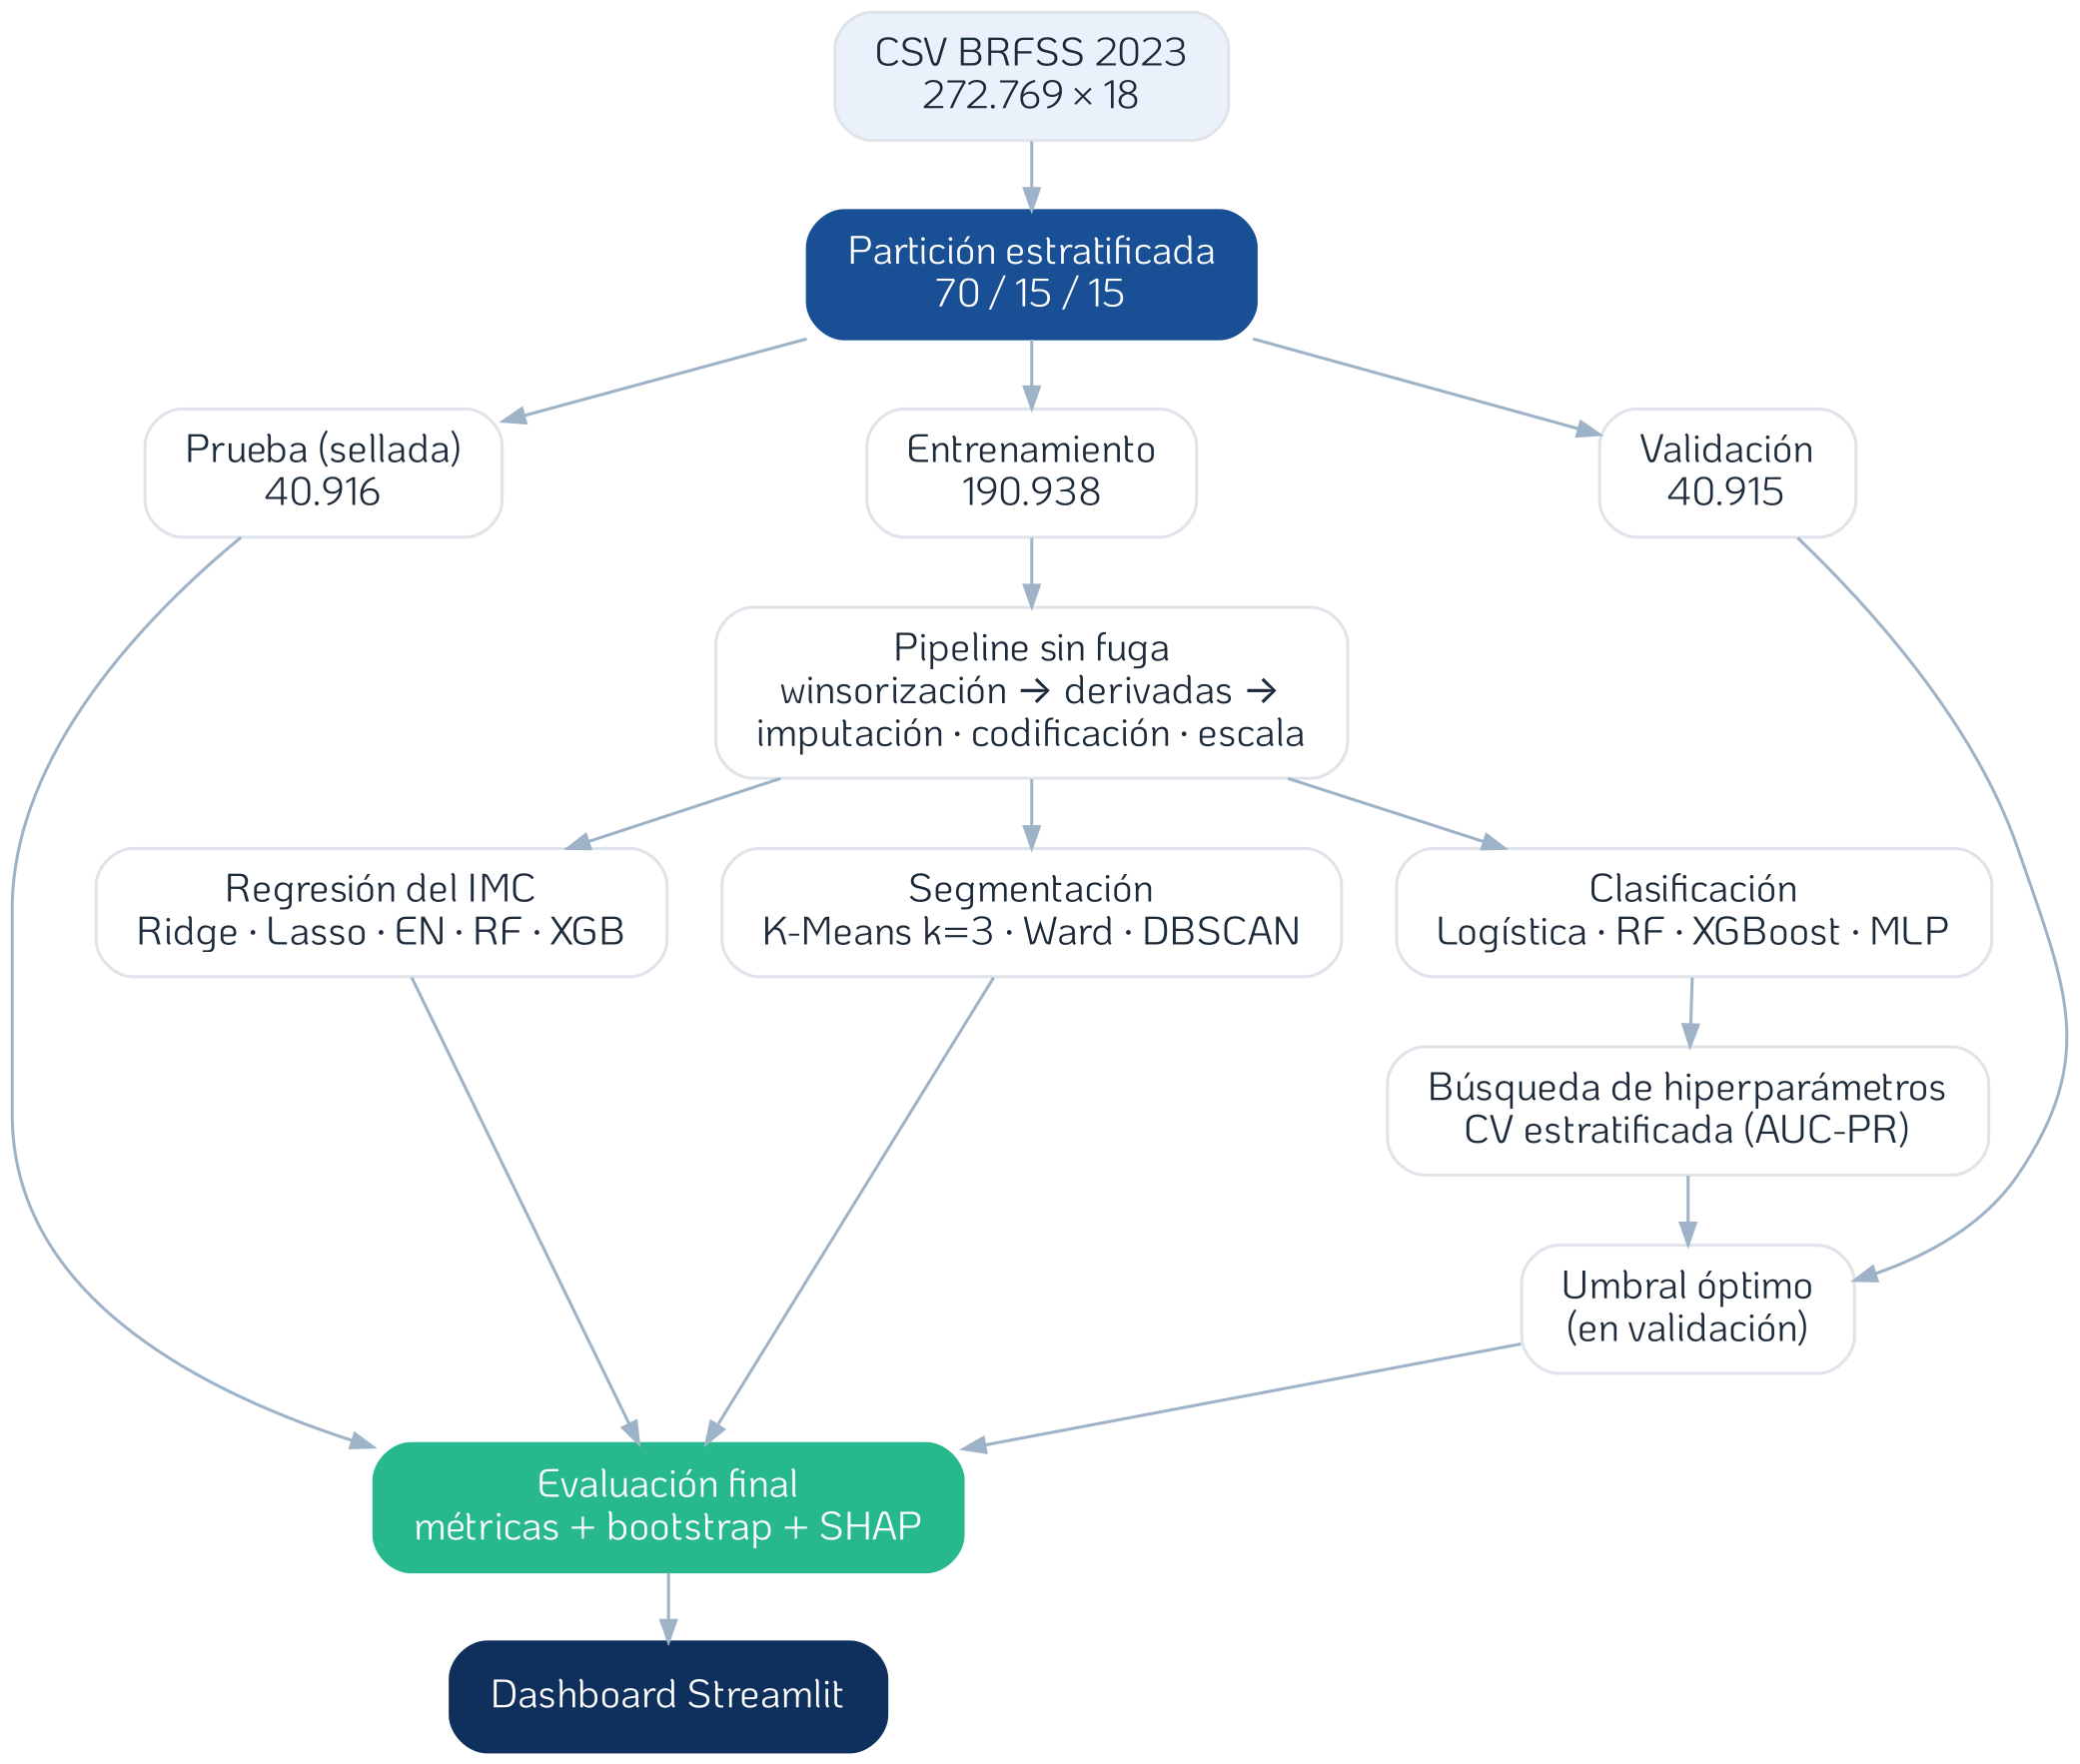
\includegraphics[width=0.86\columnwidth]{figuras/flujo_metodologico.png}
\caption{Flujo metodológico: la partición precede a toda transformación y la prueba permanece sellada.}
\label{fig:flujo}
\end{figure}

\subsection{Datos y tipología de las variables}
Se usó la versión 2023 del conjunto \textit{Diabetes Health Indicators} de Kaggle \cite{vanthieu2024}, derivado de la BRFSS \cite{cdc2023}: 272.769 registros y 18 variables enteras, sin faltantes. La variable objetivo de clasificación es el diagnóstico de diabetes o prediabetes (prevalencia de 14,6\,\%); el IMC es objetivo de la regresión y predictor de la clasificación. Aunque todas las variables se almacenan como enteros, su naturaleza estadística difiere y determina su tratamiento (Tabla~\ref{tab:variables}): once son nominales binarias, cuatro ordinales y tres cuantitativas.

\begin{table}[!t]
\centering
\caption{Diccionario de variables según tipo, rol y codificación}
\label{tab:variables}
\scriptsize
\setlength{\tabcolsep}{3pt}
\begin{tabularx}{\columnwidth}{@{}>{\raggedright\arraybackslash}p{2.35cm}>{\raggedright\arraybackslash}p{1.75cm}>{\raggedright\arraybackslash}X@{}}
\toprule
\textbf{Variable} & \textbf{Tipo} & \textbf{Rol y codificación} \\
\midrule
Diabetes\_binary & Nominal binaria & Objetivo (clasificación); 0 no, 1 sí \\
BMI & Cuantitativa continua (razón) & Objetivo (regresión) y predictor; 12--100 kg/m$^2$ \\
HighBP, HighChol, CholCheck & Nominal binaria & Predictores; 0 no, 1 sí \\
Smoker, Stroke, HeartDiseaseorAttack & Nominal binaria & Predictores; 0 no, 1 sí \\
PhysActivity, NoDocbcCost, DiffWalk & Nominal binaria & Predictores; 0 no, 1 sí \\
Sex & Nominal binaria & Predictor; 0 femenino, 1 masculino \\
GenHlth & Ordinal & Predictor; 1 excelente \ldots\ 5 mala \\
Age & Ordinal & Predictor; 1 (18--24) \ldots\ 13 ($\geq$80) \\
Education & Ordinal & Predictor; códigos presentes 2, 4, 5, 6 \\
Income & Ordinal & Predictor; códigos presentes 1--7 \\
MentHlth, PhysHlth & Cuantitativa discreta (conteo) & Predictores; 0--30 días \\
\midrule
CardioRisk & Derivada (conteo) & Suma de 4 condiciones (0--4) \\
UnhealthyDays & Derivada & $\min(30,\ \text{MentHlth}+\text{PhysHlth})$ \\
Age\_BMI & Derivada & Interacción edad $\times$ IMC \\
\bottomrule
\end{tabularx}
\end{table}

Se encontraron 33.805 registros repetidos (12,4\,\%). Se conservaron: con 18 variables discretas, dos personas distintas pueden compartir el mismo perfil, y los repetidos tienen una prevalencia de 2,3\,\% frente a 16,4\,\% en el resto, de modo que eliminarlos sesgaría la muestra.

\subsection{Entorno y herramientas}
El proyecto se implementó en Python~3.13 con pandas~3.0.5 y NumPy~2.5.3 para la manipulación de datos; scikit-learn~1.9.1 \cite{pedregosa2011} para \textit{pipelines}, modelos clásicos, agrupamiento y métricas; imbalanced-learn~0.14.2 \cite{lemaitre2017}; XGBoost~3.4.1 \cite{chen2016}; PyTorch~2.15.0 \cite{paszke2019}; SHAP~0.54.1 \cite{lundberg2017}; SciPy~1.18.1; matplotlib y seaborn para figuras estáticas, y Streamlit~1.67 con Plotly~7.1 para la aplicación. Los cuadernos se construyeron con \texttt{nbformat} y se ejecutaron de principio a fin con \texttt{nbclient}, de modo que cada resultado proviene de una ejecución completa. Las versiones exactas se fijaron en \texttt{requirements.txt} y \texttt{environment.yml}.

\subsection{Datos faltantes y valores atípicos}
Como no hay faltantes reales, el tratamiento se evaluó por simulación sobre el IMC: se ocultó cerca del 10\,\% de los valores de entrenamiento bajo los mecanismos MCAR, MAR (condicionado a edad y salud percibida) y MNAR (ocultando con mayor probabilidad los IMC altos) \cite{little2019}, y se midió el error de cuatro imputadores (Tabla~\ref{tab:imputacion}).

\begin{table}[!t]
\centering
\caption{Error de reconstrucción del IMC por mecanismo e imputador}
\label{tab:imputacion}
\scriptsize
\begin{tabular}{@{}llrr@{}}
\toprule
\textbf{Mecanismo} & \textbf{Imputador} & \textbf{RMSE} & \textbf{Sesgo} \\
\midrule
MCAR & Media & 6{,}32 & 0{,}20 \\
MCAR & Mediana & 6{,}34 & -0{,}53 \\
MCAR & KNNImputer ($k=5$) & 6{,}41 & 0{,}26 \\
MCAR & IterativeImputer & 5{,}91 & 0{,}20 \\
MAR & Media & 6{,}81 & -0{,}75 \\
MAR & Mediana & 7{,}18 & -2{,}38 \\
MAR & KNNImputer ($k=5$) & 6{,}82 & -0{,}09 \\
MAR & IterativeImputer & 6{,}36 & -0{,}22 \\
MNAR & Media & 12{,}60 & -9{,}49 \\
MNAR & Mediana & 13{,}22 & -10{,}31 \\
MNAR & KNNImputer ($k=5$) & 11{,}75 & -8{,}46 \\
MNAR & IterativeImputer & 11{,}73 & -8{,}74 \\
\bottomrule

\end{tabular}\\[2pt]
{\footnotesize RMSE y sesgo en kg/m$^2$; sesgo = media(imputado $-$ real).}
\end{table}

IterativeImputer minimizó el error bajo MCAR y MAR; bajo MNAR todos los métodos fallan (sesgos cercanos a $-9$~kg/m$^2$), porque lo oculto no es predecible desde lo observado. Se dejó un \texttt{SimpleImputer} de mediana en el \textit{pipeline} como salvaguarda para datos nuevos. Para los atípicos del IMC se compararon cuatro alternativas (Tabla~\ref{tab:atipicos}). La remoción por rango intercuartílico eliminaría el 2,54\,\% de los registros, con una prevalencia de diabetes de 31,9\,\%; se adoptó la winsorización p1--p99 (18 y 50~kg/m$^2$), que reduce la curtosis de 4,19 a 1,09 sin perder registros.

\begin{table}[!t]
\centering
\caption{Alternativas para los valores extremos del IMC}
\label{tab:atipicos}
\scriptsize
\begin{tabular}{@{}lrrrr@{}}
\toprule
\textbf{Alternativa} & \textbf{Media} & \textbf{D.E.} & \textbf{Curtosis} & \textbf{\% elim.} \\
\midrule
Original & 28{,}81 & 6{,}52 & 4{,}19 & 0{,}00 \\
Winsorización p1--p99 & 28{,}76 & 6{,}23 & 1{,}09 & 0{,}00 \\
Transformación logarítmica & 3{,}34 & 0{,}21 & 0{,}68 & 0{,}00 \\
Remoción por regla IQR & 28{,}24 & 5{,}48 & 0{,}01 & 2{,}54 \\
\bottomrule

\end{tabular}
\end{table}

\subsection{Ingeniería de variables y \textit{pipeline} sin fuga}
Se crearon cuatro variables con justificación clínica (Tabla~\ref{tab:variables}) y la categoría de IMC de la OMS. Las ordinales se codificaron con su orden natural declarando las categorías válidas, la categoría de IMC con \textit{One-Hot} (sin la primera) y las numéricas se estandarizaron. CardioRisk se excluyó de los modelos lineales por ser combinación lineal exacta de cuatro predictores. Todas las transformaciones viven dentro de un \texttt{Pipeline} (Listado~\ref{lst:pipe}), de modo que en cada pliegue de validación cruzada los percentiles, medianas, codificaciones y medias del escalador se reajustan solo con la parte de entrenamiento del pliegue \cite{kaufman2012}. El mismo código vive en \texttt{src/preprocesamiento.py}, que comparten el reentrenamiento y la aplicación.

\begin{lstlisting}[caption={Extracto de \texttt{src/preprocesamiento.py}}, label={lst:pipe}]
class Winsorizer(BaseEstimator, TransformerMixin):
    def fit(self, X, y=None):   # solo entrenamiento
        self.limites_ = {c: (X[c].quantile(.01),
                             X[c].quantile(.99))
                         for c in self.columnas}
        return self
    def transform(self, X):
        X = X.copy()
        for c, (lo, hi) in self.limites_.items():
            X[c] = X[c].clip(lo, hi)
        return X

def pipe_arbol_clf(modelo):     # XGBoost y RF
    return Pipeline([
        ("recorte", Winsorizer()),
        ("derivadas", FunctionTransformer(vars_arbol)),
        ("modelo", modelo)])
\end{lstlisting}

\subsection{Partición y desbalance}
Los datos se dividieron con \texttt{train\_test\_split} estratificado y semilla fija en entrenamiento (190.938), validación (40.915) y prueba (40.916). La razón de clases es 5,84:1. La Tabla~\ref{tab:desbalance} compara estrategias en validación con una regresión logística.

\begin{table}[!t]
\centering
\caption{Estrategias de desbalance (regresión logística, validación)}
\label{tab:desbalance}
\scriptsize
\setlength{\tabcolsep}{4pt}
\begin{tabular}{@{}lrrrrr@{}}
\toprule
\textbf{Estrategia} & \textbf{Exact.} & \textbf{Prec.} & \textbf{Sens.} & \textbf{F1} & \textbf{AUC-PR} \\
\midrule
Sin tratamiento & 0{,}857 & 0{,}546 & 0{,}145 & 0{,}229 & 0{,}403 \\
Pesos de clase & 0{,}718 & 0{,}309 & 0{,}751 & 0{,}438 & 0{,}402 \\
SMOTE & 0{,}718 & 0{,}309 & 0{,}751 & 0{,}438 & 0{,}397 \\
Submuestreo & 0{,}718 & 0{,}309 & 0{,}752 & 0{,}438 & 0{,}402 \\
Umbral (0,22) & 0{,}787 & 0{,}361 & 0{,}594 & 0{,}449 & 0{,}403 \\
\bottomrule

\end{tabular}
\end{table}

Sin tratamiento, la exactitud es la mayor (0,857) pero solo se detecta el 14,5\,\% de los casos. Pesos de clase, SMOTE \cite{chawla2002} y submuestreo rinden igual; se eligieron los pesos de clase porque no generan registros sintéticos ni descartan información. En XGBoost equivalen a \texttt{scale\_pos\_weight}~$=5{,}84$ y en la red neuronal al parámetro \texttt{pos\_weight} de la pérdida.

\subsection{Formulación de los modelos supervisados}
La regresión logística estima $p=\sigma(\beta_0+\boldsymbol\beta^\top\mathbf x)$ minimizando la entropía cruzada ponderada, con $w_1=n_0/n_1$:
\begin{equation}
\mathcal L(\boldsymbol\beta)=-\sum_i\big[w_1 y_i\log p_i+(1-y_i)\log(1-p_i)\big]+\lambda\lVert\boldsymbol\beta\rVert_2^2 .
\end{equation}
Para el IMC, Ridge, Lasso y ElasticNet \cite{hoerl1970,tibshirani1996,zou2005} penalizan los mínimos cuadrados, con $\alpha$ elegido por validación cruzada de cinco pliegues:
\begin{equation}
\min_{\boldsymbol\beta}\ \lVert\mathbf y-\mathbf X\boldsymbol\beta\rVert_2^2+\alpha\Big[\rho\lVert\boldsymbol\beta\rVert_1+\tfrac{1-\rho}{2}\lVert\boldsymbol\beta\rVert_2^2\Big].
\end{equation}
Random Forest promedia árboles entrenados sobre muestras \textit{bootstrap} y subconjuntos aleatorios de variables \cite{breiman2001}. XGBoost ajusta árboles aditivos $f_k$ al gradiente de la pérdida y regulariza su complejidad \cite{chen2016}:
\begin{equation}
\text{Obj}=\sum_i \ell(y_i,\hat y_i)+\sum_k\Big[\gamma T_k+\tfrac12\lambda\lVert\mathbf w_k\rVert^2\Big],
\end{equation}
con $\hat y_i=\sum_k f_k(\mathbf x_i)$,
donde $T_k$ es el número de hojas del árbol $k$ y $\mathbf w_k$ sus pesos. El perceptrón multicapa (PyTorch) tiene arquitectura 24--64--32--1 con ReLU, \textit{dropout} de 0,2 \cite{srivastava2014}, 3.713 parámetros, pérdida \texttt{BCEWithLogitsLoss} con \texttt{pos\_weight}~$=5{,}84$, optimizador Adam \cite{kingma2015} (tasa $10^{-3}$, decaimiento $10^{-4}$), lotes de 1.024, máximo 60 épocas y parada temprana con paciencia de 6 épocas restaurando los mejores pesos \cite{prechelt1998}.

\subsection{Optimización de hiperparámetros}
Los ensambles se ajustaron con \texttt{RandomizedSearchCV} \cite{bergstra2012} y validación cruzada estratificada de tres pliegues, con el \textit{pipeline} completo dentro de cada pliegue, maximizando el AUC-PR en clasificación y minimizando el RMSE en regresión. Para XGBoost se exploraron 15 de las 5.184 combinaciones de \texttt{n\_estimators}, \texttt{max\_depth}, \texttt{learning\_rate}, \texttt{subsample}, \texttt{colsample\_bytree}, \texttt{min\_child\_weight} y \texttt{reg\_lambda}; para Random Forest, 6 de 36 combinaciones de profundidad, tamaño mínimo de hoja y fracción de variables.

\subsection{Métricas y protocolo de evaluación}
Con $TP$, $FP$, $FN$ y $TN$ se reportan precisión, sensibilidad, especificidad y
\begin{equation}
F_1=\frac{2\cdot\text{Precisión}\cdot\text{Sensibilidad}}{\text{Precisión}+\text{Sensibilidad}} .
\end{equation}
El AUC-PR es más informativo que el AUC-ROC con clases desbalanceadas porque su línea base es la prevalencia \cite{saito2015}. En regresión se usan R$^2$, RMSE y MAE. El umbral que maximiza $F_1$ se eligió en validación. Los intervalos de confianza del 95\,\% y las diferencias entre modelos se estimaron con \textit{bootstrap} (pareado) de 400 remuestreos del conjunto de prueba \cite{efron1993}.

\subsection{Aprendizaje no supervisado}
Se usaron ocho variables estandarizadas (IMC recortado, edad, salud general, días de malestar físico y mental, educación, ingreso y CardioRisk), sin la variable objetivo. K-Means \cite{macqueen1967} minimiza la inercia $J=\sum_k\sum_{\mathbf x_i\in C_k}\lVert\mathbf x_i-\boldsymbol\mu_k\rVert^2$; $k\in\{2,\ldots,8\}$ se evaluó con el codo y la silueta \cite{rousseeuw1987}
\begin{equation}
s(i)=\frac{b(i)-a(i)}{\max\{a(i),b(i)\}},
\end{equation}
calculada sobre 15.000 registros. DBSCAN \cite{ester1996} usó \texttt{min\_samples}~$=16$ y cinco valores de $\varepsilon$ guiados por el gráfico de distancias $k$-vecinos; Ward \cite{ward1963} se ajustó sobre 8.000 registros. La concordancia se midió con el índice de Rand ajustado (ARI) \cite{hubert1985} y la asociación clúster--diabetes con $\chi^2$ y la V de Cramér. Un PCA de tres componentes, ajustado con entrenamiento, se usa para visualizar.

\subsection{Interpretabilidad}
El valor SHAP de la variable $j$ es su valor de Shapley \cite{shapley1953,lundberg2017}:
\begin{equation}
\phi_j=\sum_{S\subseteq F\setminus\{j\}}\frac{|S|!\,(|F|-|S|-1)!}{|F|!}\big[f(S\cup\{j\})-f(S)\big].
\end{equation}
TreeSHAP lo calcula de forma exacta en tiempo polinómico para árboles \cite{lundberg2020}. La importancia global es la media de $|\phi_j|$ en validación; como contraste independiente del modelo se calculó la importancia por permutación. En la aplicación, las explicaciones individuales usan \texttt{pred\_contribs} de XGBoost, que implementa el mismo algoritmo.

\subsection{Ingeniería de software y aplicación web}
La Fig.~\ref{fig:arq} muestra la arquitectura del repositorio. El script \texttt{src/entrenar\_modelos.py} reproduce la partición, reentrena los modelos finales con los hiperparámetros elegidos, los serializa con \texttt{joblib} y genera los datos de la aplicación en formato \textit{parquet}; su ejecución reproduce exactamente las métricas de prueba de la Fase~3.

\begin{figure*}[!t]
\centering
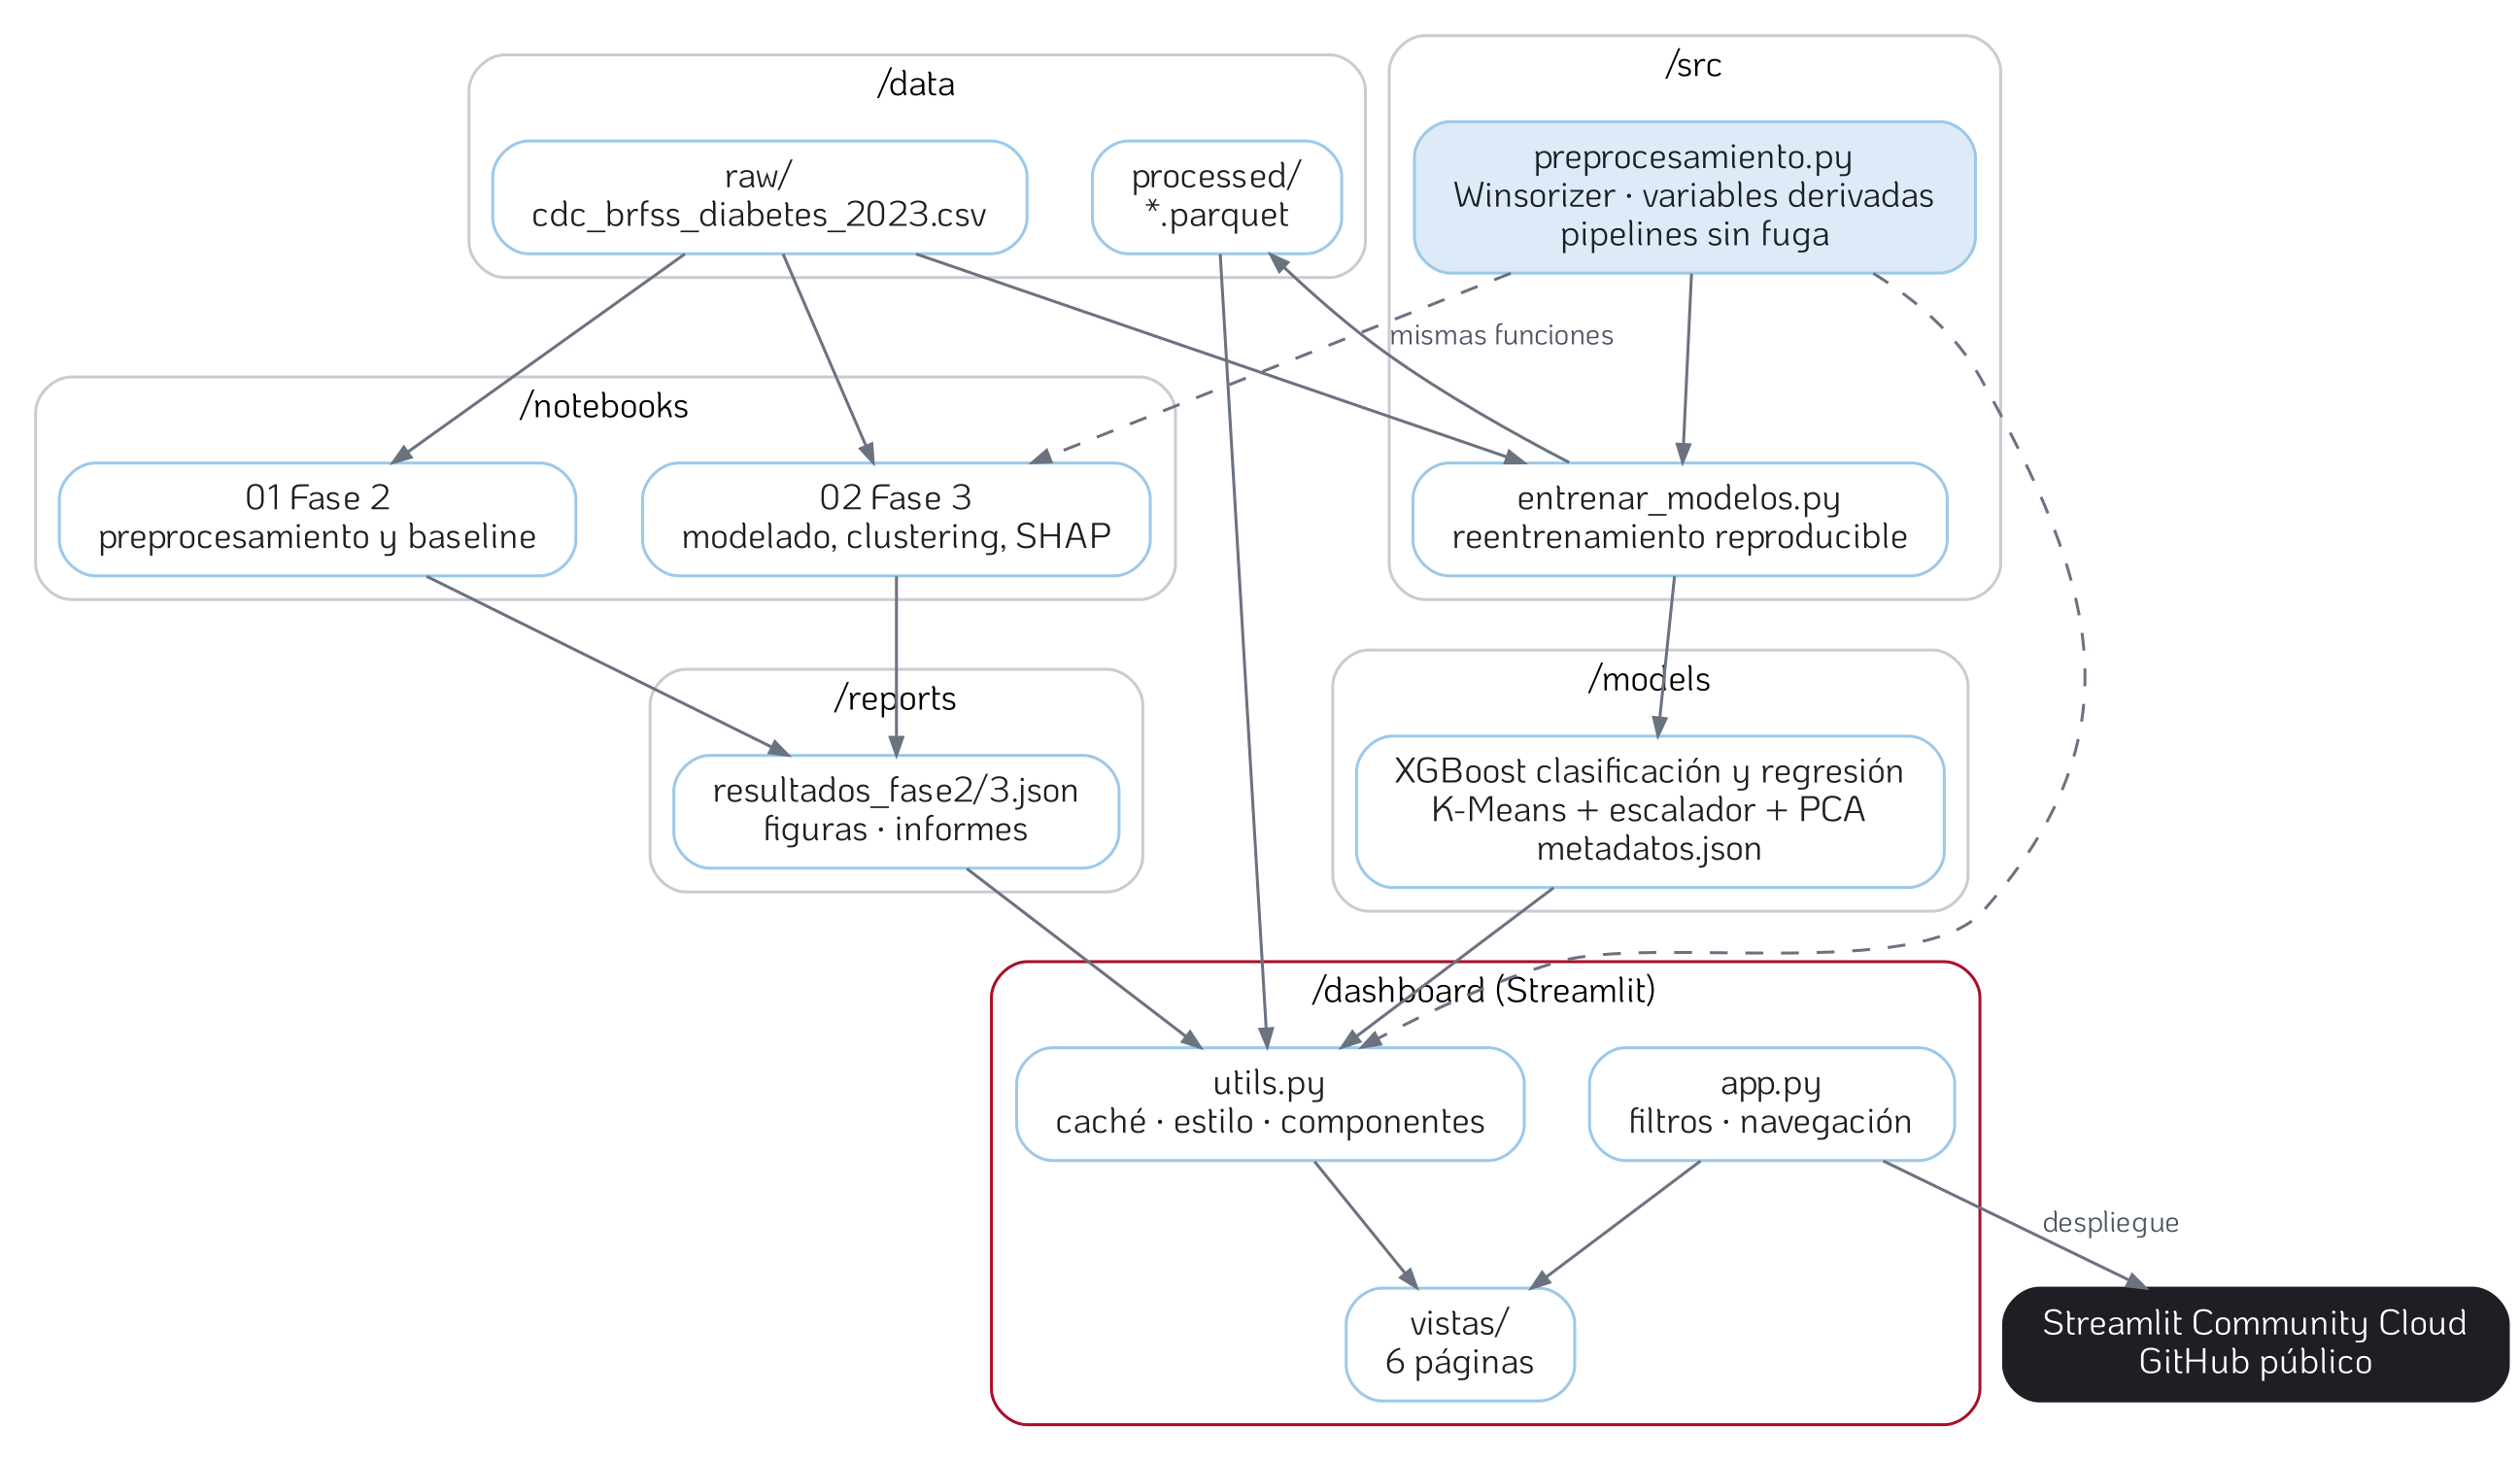
\includegraphics[width=0.78\textwidth]{figuras/arquitectura_software.png}
\caption{Arquitectura del repositorio y de la aplicación: el módulo \texttt{src/preprocesamiento.py} es compartido por el reentrenamiento y la aplicación.}
\label{fig:arq}
\end{figure*}

La aplicación es un tablero multipágina de Streamlit con gráficos Plotly. Los datos y modelos se cargan una vez con \texttt{st.cache\_data} y \texttt{st.cache\_resource}; los filtros se guardan en el estado de sesión. Cubre los cuatro módulos exigidos: (1) \textbf{filtros dinámicos} por año, rangos de edad e IMC y categorías (sexo, salud, ingreso, educación, condiciones, perfil y diagnóstico), más selección cruzada entre gráficos; (2) \textbf{tarjetas KPI} animadas de la población y del rendimiento del modelo; (3) \textbf{predicción en vivo} con indicador de riesgo, ubicación en la distribución, cascada SHAP y escenarios contrafactuales, y (4) \textbf{segmentación} con dispersión 3D/2D en el espacio PCA y perfiles promedio. La calidad se verificó con pruebas automatizadas (\texttt{AppTest}) de las seis páginas bajo filtros extremos (de la población completa a seis personas), instalación en un entorno limpio y capturas automáticas con un navegador sin interfaz.

% =====================================================================
\section{Resultados}
% =====================================================================
\subsection{Gradientes de riesgo}
La prevalencia crece de forma escalonada (Fig.~\ref{fig:derivadas}): de 4,3\,\% sin condiciones cardiometabólicas a 45,3\,\% con las cuatro, y de 7,0\,\% con peso normal a 30,2\,\% con obesidad grado~III. La correlación de Spearman de CardioRisk con la diabetes (0,295) supera a la de cualquiera de sus componentes (la mayor, hipertensión, 0,256). En el conjunto completo, la prevalencia es de 24,7\,\% en el nivel de ingreso más bajo y de 6,5\,\% en el más alto.

\begin{figure*}[!t]
\centering
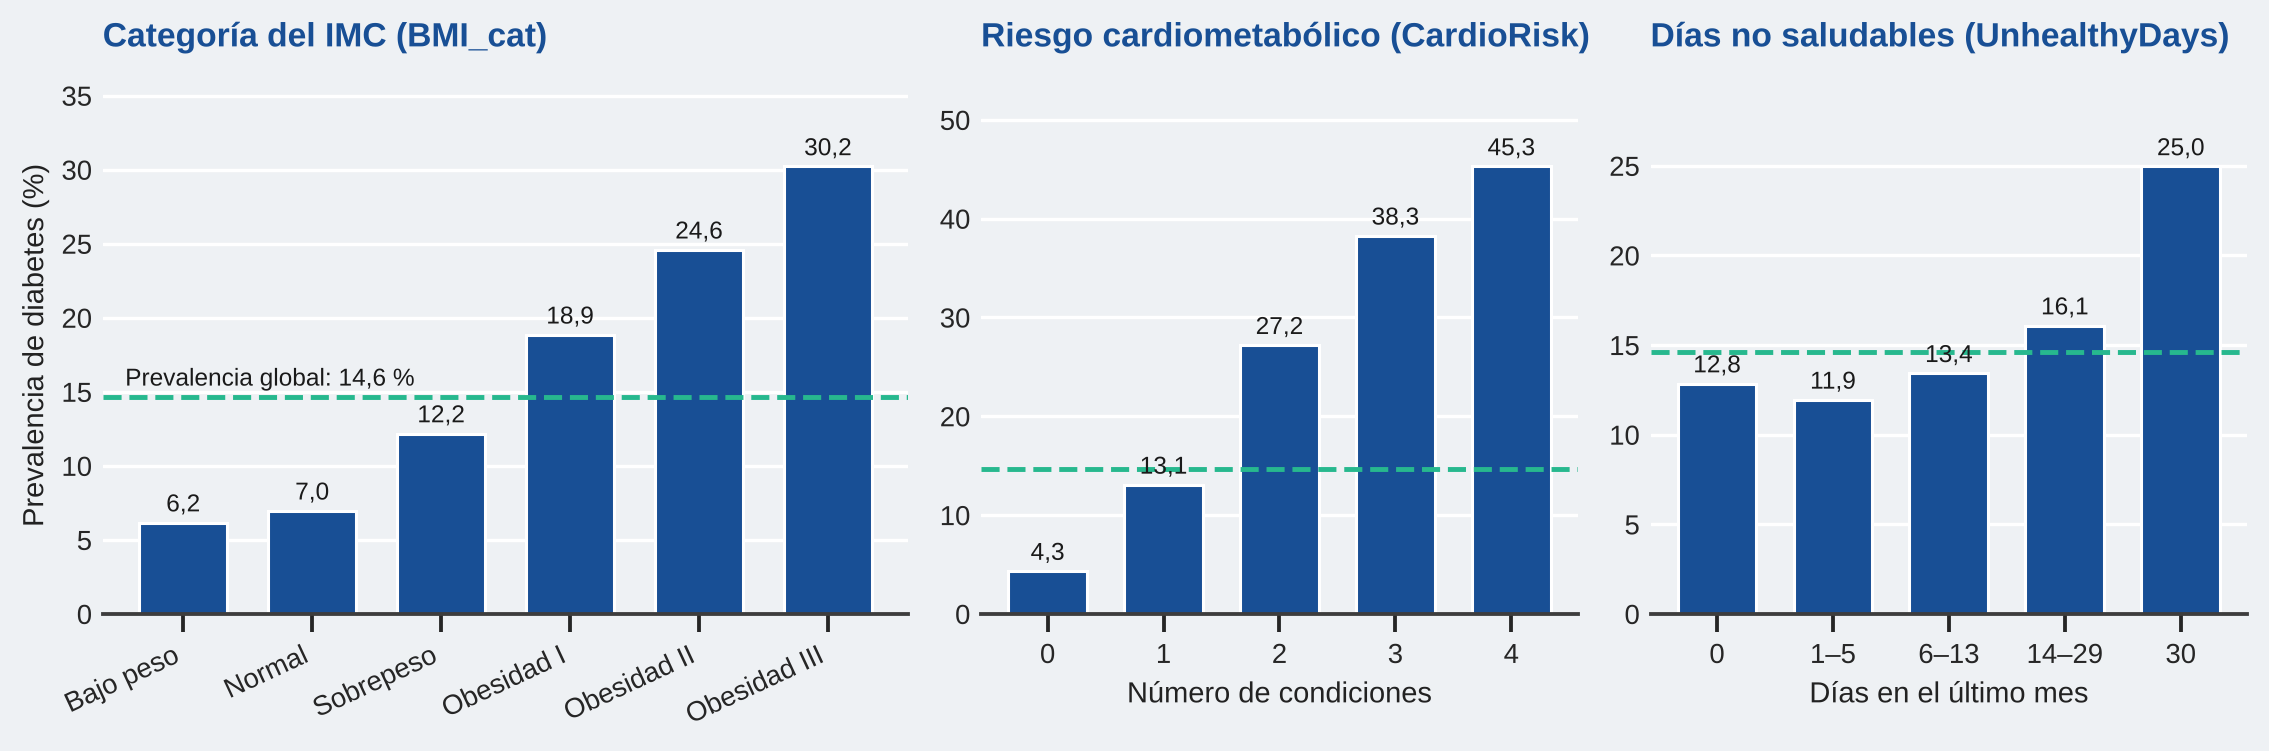
\includegraphics[width=0.82\textwidth]{figuras/fig3_derivadas.png}
\caption{Prevalencia de diabetes según las variables derivadas (conjunto de entrenamiento).}
\label{fig:derivadas}
\end{figure*}

\subsection{Modelos de referencia y ablación}
El clasificador de clase mayoritaria obtiene 85,4\,\% de exactitud sin detectar un solo caso (Tabla~\ref{tab:base}). La ablación (Tabla~\ref{tab:ablacion}) muestra que, en el modelo lineal, las variables derivadas mejoran el AUC-PR en apenas 0,0014 y que entrenar sin duplicados no cambia el resultado; en cambio, en los árboles dos de ellas están entre las tres variables más influyentes (Sección~\ref{sec:shap}).

\begin{table}[!t]
\centering
\caption{Modelos de referencia (validación)}
\label{tab:base}
\scriptsize
\setlength{\tabcolsep}{4pt}
\begin{tabular}{@{}lrrrrr@{}}
\toprule
\textbf{Modelo} & \textbf{Exact.} & \textbf{Sens.} & \textbf{F1} & \textbf{ROC} & \textbf{PR} \\
\midrule
Dummy mayoritario & 0{,}854 & 0{,}000 & 0{,}000 & 0{,}500 & 0{,}146 \\
Dummy estratificado & 0{,}752 & 0{,}148 & 0{,}149 & 0{,}502 & 0{,}147 \\
Regresión logística & 0{,}718 & 0{,}751 & 0{,}438 & 0{,}807 & 0{,}402 \\
\bottomrule

\end{tabular}
\end{table}

\begin{table}[!t]
\centering
\caption{Ablación del preprocesamiento (regresión logística, validación)}
\label{tab:ablacion}
\scriptsize
\setlength{\tabcolsep}{4pt}
\begin{tabular}{@{}lrrrr@{}}
\toprule
\textbf{Variante} & \textbf{Sens.} & \textbf{F1} & \textbf{ROC} & \textbf{PR} \\
\midrule
Solo originales (17) & 0{,}753 & 0{,}437 & 0{,}806 & 0{,}400 \\
Con derivadas (24) & 0{,}751 & 0{,}438 & 0{,}807 & 0{,}402 \\
Con derivadas, sin duplicados & 0{,}746 & 0{,}440 & 0{,}806 & 0{,}400 \\
\bottomrule

\end{tabular}
\end{table}

\subsection{Clasificación}
Con hiperparámetros iniciales (Tabla~\ref{tab:inicial}), los ensambles superan por poco a la regresión logística en validación; Random Forest muestra la mayor brecha entre entrenamiento y validación. La búsqueda de hiperparámetros (Tabla~\ref{tab:hiper}) produjo ganancias menores que la variación entre pliegues y favoreció configuraciones más regularizadas:
\begin{itemize}
\item \textbf{XGBoost (clasificación)}: \texttt{colsample\_bytree = 0{,}8, learning\_rate = 0{,}03, max\_depth = 5, min\_child\_weight = 1, n\_estimators = 400, reg\_lambda = 10, subsample = 0{,}7}
\item \textbf{Random Forest (clasificación)}: \texttt{max\_depth = None, max\_features = 0{,}3, min\_samples\_leaf = 20}
\item \textbf{XGBoost (regresión)}: \texttt{colsample\_bytree = 0{,}6, learning\_rate = 0{,}03, max\_depth = 6, min\_child\_weight = 1, n\_estimators = 400, reg\_lambda = 5, subsample = 0{,}85}

\end{itemize}

\begin{table}[!t]
\centering
\caption{Clasificadores con hiperparámetros iniciales}
\label{tab:inicial}
\scriptsize
\setlength{\tabcolsep}{4pt}
\begin{tabular}{@{}llrrrr@{}}
\toprule
\textbf{Modelo} & \textbf{Conj.} & \textbf{F1} & \textbf{ROC} & \textbf{PR} & \textbf{t (s)} \\
\midrule
Regresión logística & Entr. & 0{,}441 & 0{,}810 & 0{,}402 & 0{,}9 \\
Regresión logística & Val. & 0{,}438 & 0{,}807 & 0{,}402 & 0{,}9 \\
Random Forest & Entr. & 0{,}467 & 0{,}836 & 0{,}458 & 6{,}5 \\
Random Forest & Val. & 0{,}442 & 0{,}809 & 0{,}416 & 6{,}5 \\
XGBoost & Entr. & 0{,}446 & 0{,}824 & 0{,}432 & 2{,}9 \\
XGBoost & Val. & 0{,}435 & 0{,}813 & 0{,}423 & 2{,}9 \\
\bottomrule

\end{tabular}
\end{table}

\begin{table}[!t]
\centering
\caption{Búsqueda de hiperparámetros con validación cruzada}
\label{tab:hiper}
\scriptsize
\setlength{\tabcolsep}{4pt}
\begin{tabular}{@{}llrrrr@{}}
\toprule
\textbf{Modelo} & \textbf{Métrica} & \textbf{Inicial} & \textbf{Óptimo} & \textbf{D.E.} & \textbf{t (s)} \\
\midrule
XGB clasif. & AUC-PR & 0{,}4153 & 0{,}4164 & 0{,}0026 & 139 \\
RF clasif. & AUC-PR & 0{,}4100 & 0{,}4108 & 0{,}0037 & 60 \\
XGB regres. & RMSE & 5{,}5924 & 5{,}5901 & 0{,}0107 & 102 \\
\bottomrule

\end{tabular}\\[2pt]
{\footnotesize D.E.: desviación entre pliegues de la configuración óptima.}
\end{table}

La Tabla~\ref{tab:prueba} presenta el desempeño final en prueba. Las cuatro familias convergen (AUC-ROC entre 0,810 y 0,816). XGBoost supera a la regresión logística en 0,0056 de AUC-ROC (IC~95\,\% pareado: 0,0041--0,0071) y en 0,0142 de AUC-PR (0,0089--0,0192): diferencias estadísticamente distinguibles, pero pequeñas. El perceptrón multicapa iguala a XGBoost, en línea con \cite{grinsztajn2022}. Se desplegó XGBoost por su mejor AUC-PR y por admitir explicaciones SHAP exactas.

\begin{table}[!t]
\centering
\caption{Clasificadores en el conjunto de prueba ($n=40.916$)}
\label{tab:prueba}
\scriptsize
\setlength{\tabcolsep}{3.2pt}
\begin{tabular}{@{}lrrrrrr@{}}
\toprule
\textbf{Modelo} & \textbf{Umbral} & \textbf{Prec.} & \textbf{Sens.} & \textbf{F1} & \textbf{ROC} & \textbf{PR} \\
\midrule
Reg. logística & 0{,}50 & 0{,}313 & 0{,}749 & 0{,}441 & 0{,}810 & 0{,}399 \\
Reg. logística & 0{,}57 & 0{,}344 & 0{,}664 & 0{,}453 & 0{,}810 & 0{,}399 \\
Random Forest & 0{,}50 & 0{,}326 & 0{,}727 & 0{,}451 & 0{,}813 & 0{,}409 \\
Random Forest & 0{,}58 & 0{,}369 & 0{,}607 & 0{,}459 & 0{,}813 & 0{,}409 \\
XGBoost & 0{,}50 & 0{,}306 & 0{,}787 & 0{,}441 & 0{,}816 & 0{,}413 \\
XGBoost & 0{,}62 & 0{,}362 & 0{,}640 & 0{,}462 & 0{,}816 & 0{,}413 \\
MLP & 0{,}50 & 0{,}309 & 0{,}781 & 0{,}443 & 0{,}816 & 0{,}413 \\
MLP & 0{,}63 & 0{,}367 & 0{,}624 & 0{,}462 & 0{,}816 & 0{,}413 \\
\bottomrule

\end{tabular}\\[2pt]
{\footnotesize Cada modelo con umbral 0,5 y con el umbral que maximiza F1 en validación.}
\end{table}

Con umbral 0,5, XGBoost detecta 4.706 de las 5.982 personas con diabetes (sensibilidad 78,7\,\%, especificidad 69,5\,\%, valor predictivo positivo 30,6\,\%). Por cada 1.000 adultos tamizados, 375 irían a prueba de laboratorio, 115 de ellos con diabetes, y quedarían sin detectar 31 casos. Con el umbral óptimo (0,62), F1 sube a 0,462 y la sensibilidad baja a 64,0\,\%. El F1 máximo alcanzable con este ordenamiento es 0,464. La Fig.~\ref{fig:roc} muestra las curvas y la Fig.~\ref{fig:mlp} el entrenamiento de la red, cuyo mínimo de validación ocurrió en la época~19 (parada en la 25).

\begin{figure*}[!t]
\centering
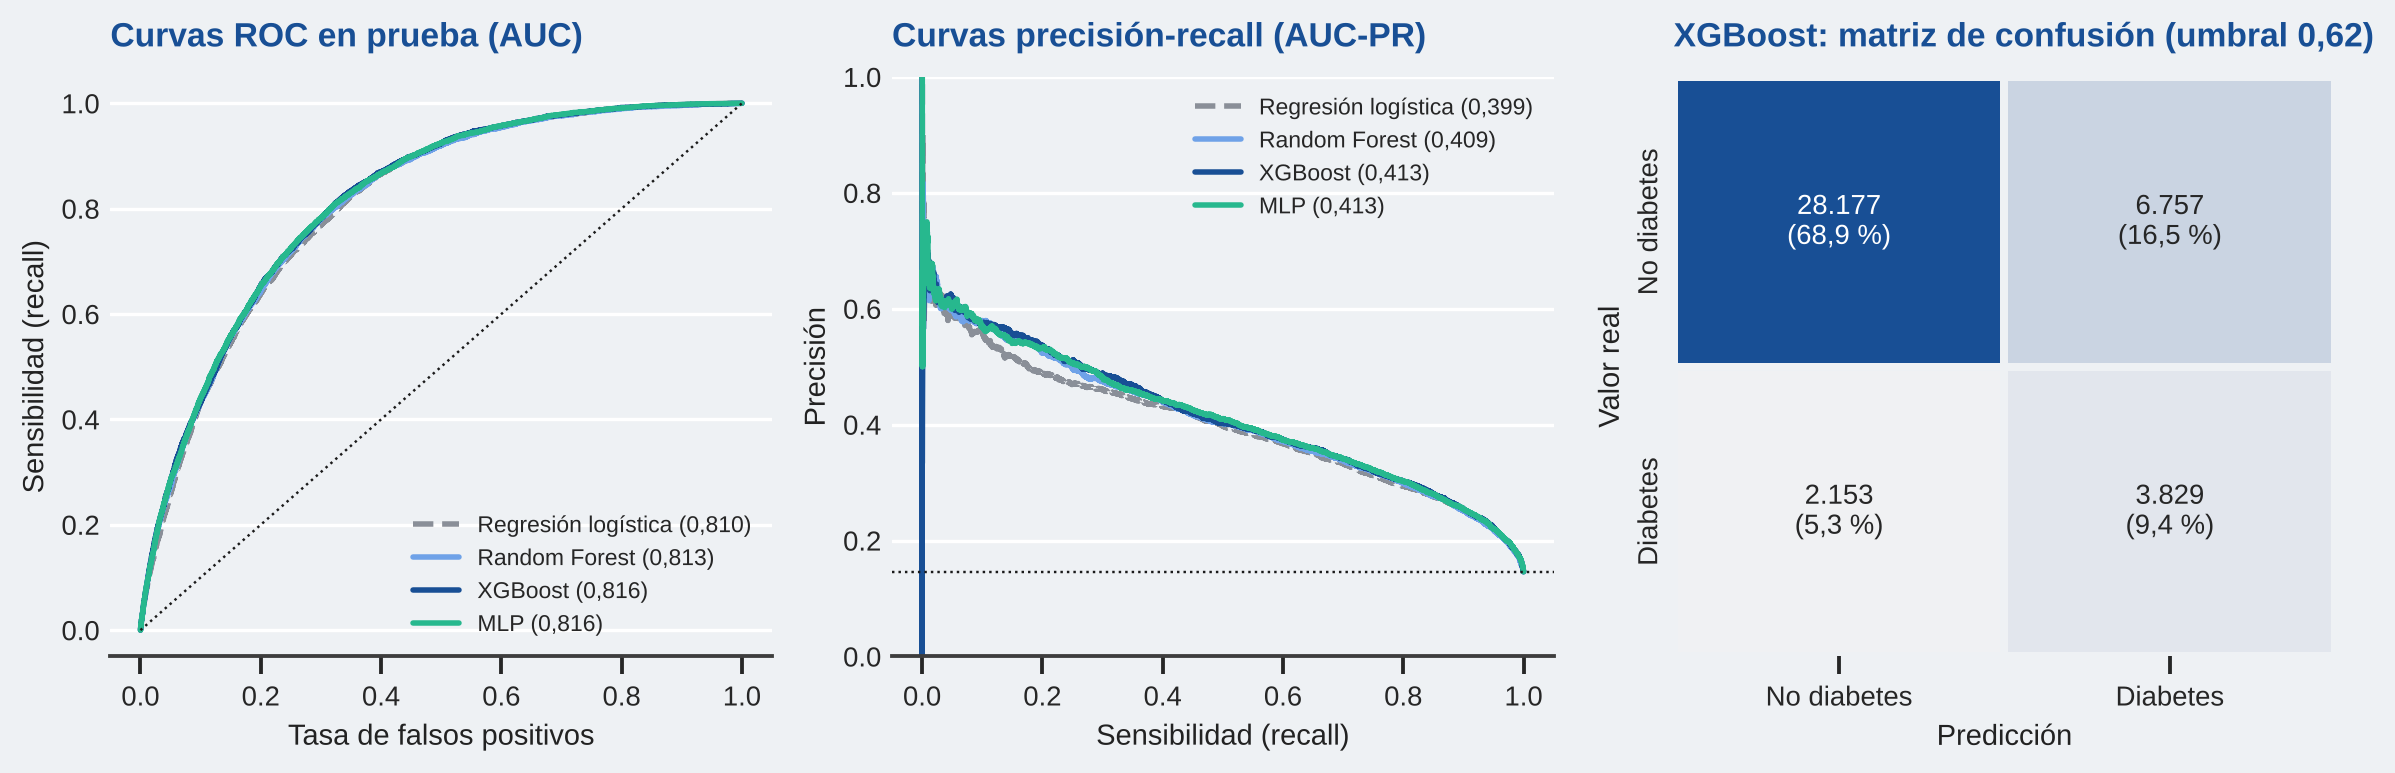
\includegraphics[width=0.9\textwidth]{figuras/fig6_test_clasificacion.png}
\caption{Curvas ROC y precisión--sensibilidad en prueba y matriz de confusión de XGBoost.}
\label{fig:roc}
\end{figure*}

\begin{figure}[!t]
\centering
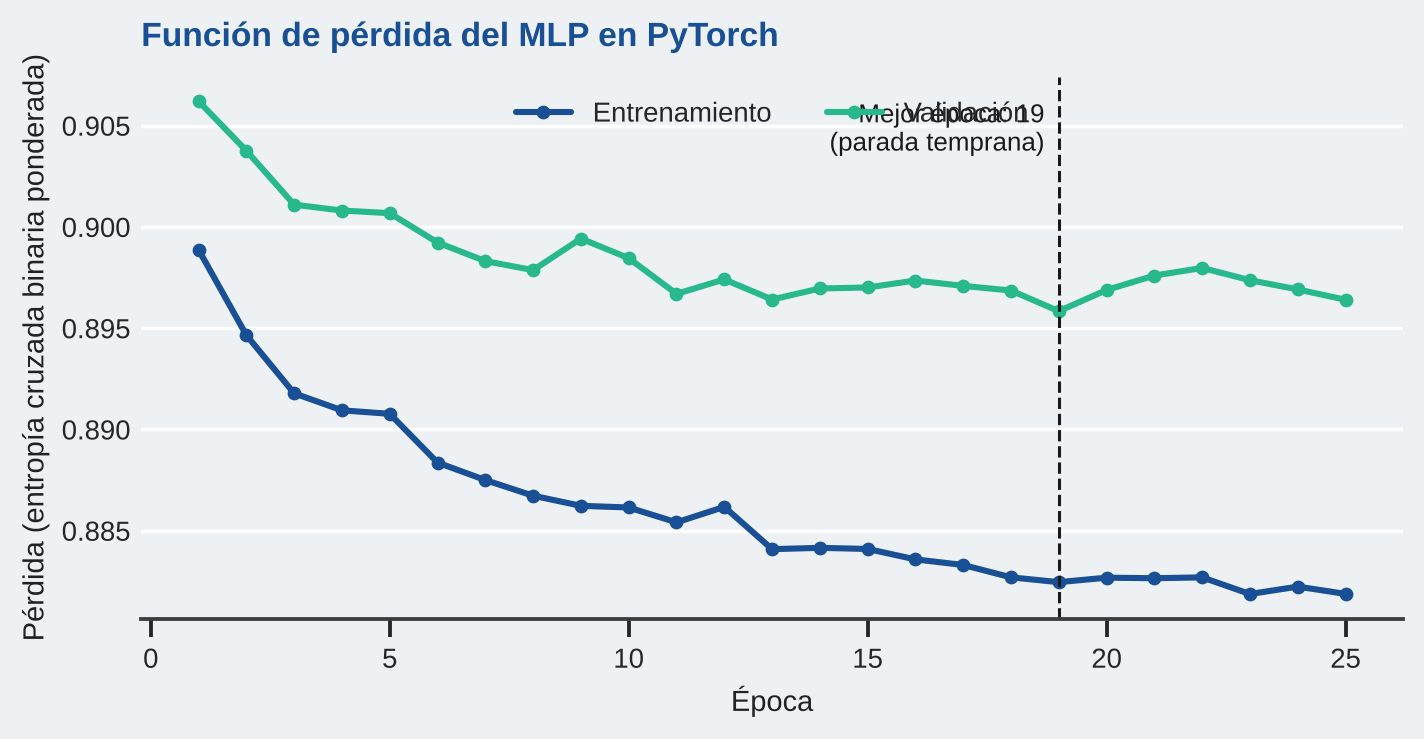
\includegraphics[width=\columnwidth]{figuras/fig5_perdida_mlp.png}
\caption{Pérdida del perceptrón multicapa en entrenamiento y validación.}
\label{fig:mlp}
\end{figure}

\subsection{Regresión del IMC}
Las regresiones regularizadas reprodujeron al modelo lineal (Tabla~\ref{tab:regresion}): con 190.938 registros y 18 predictores poco correlacionados la varianza de los coeficientes ya es mínima. Los ensambles capturaron no linealidades: en prueba, XGBoost alcanzó R$^2=0{,}186$ (IC~95\,\%: 0,178--0,193), RMSE~$=5{,}87$ y MAE~$=4{,}35$~kg/m$^2$, frente a 0,130 del modelo lineal.

\begin{table}[!t]
\centering
\caption{Regresión del IMC (entrenamiento y validación)}
\label{tab:regresion}
\scriptsize
\setlength{\tabcolsep}{4pt}
\begin{tabular}{@{}lrrrr@{}}
\toprule
\textbf{Modelo} & \textbf{R$^2$ entr.} & \textbf{R$^2$ val.} & \textbf{RMSE} & \textbf{MAE} \\
\midrule
Regresión lineal & 0{,}133 & 0{,}137 & 6{,}10 & 4{,}51 \\
Ridge & 0{,}133 & 0{,}137 & 6{,}10 & 4{,}51 \\
Lasso & 0{,}133 & 0{,}137 & 6{,}10 & 4{,}51 \\
ElasticNet & 0{,}133 & 0{,}137 & 6{,}10 & 4{,}51 \\
Random Forest & 0{,}215 & 0{,}189 & 5{,}92 & 4{,}35 \\
XGBoost & 0{,}209 & 0{,}195 & 5{,}90 & 4{,}33 \\
XGBoost (log) & 0{,}199 & 0{,}184 & 5{,}94 & 4{,}30 \\
\bottomrule

\end{tabular}
\end{table}

\subsection{Segmentación}
La silueta fue máxima con $k=2$ (0,248) y de 0,170 con $k=3$ (Fig.~\ref{fig:codo}). Se eligió $k=3$ porque distingue dos riesgos de naturaleza distinta; los valores bajos de silueta indican que la población es un continuo. DBSCAN fracasó (Tabla~\ref{tab:dbscan}): con datos discretos la densidad es casi uniforme. Ward reprodujo el orden de riesgo (ARI~$=0{,}47$), y la asociación clúster--diabetes fue significativa ($\chi^2=15.600$, $p<0{,}001$, V de Cramér~$=0{,}29$). La Tabla~\ref{tab:perfiles} y la Fig.~\ref{fig:clusters} describen los perfiles: C1, adultos jóvenes sanos; C2, adultos mayores con hipertensión y colesterol alto que reportan pocos días de malestar (riesgo «silencioso»), y C3, salud deteriorada con malestar físico y mental y el menor ingreso.

\begin{figure}[!t]
\centering
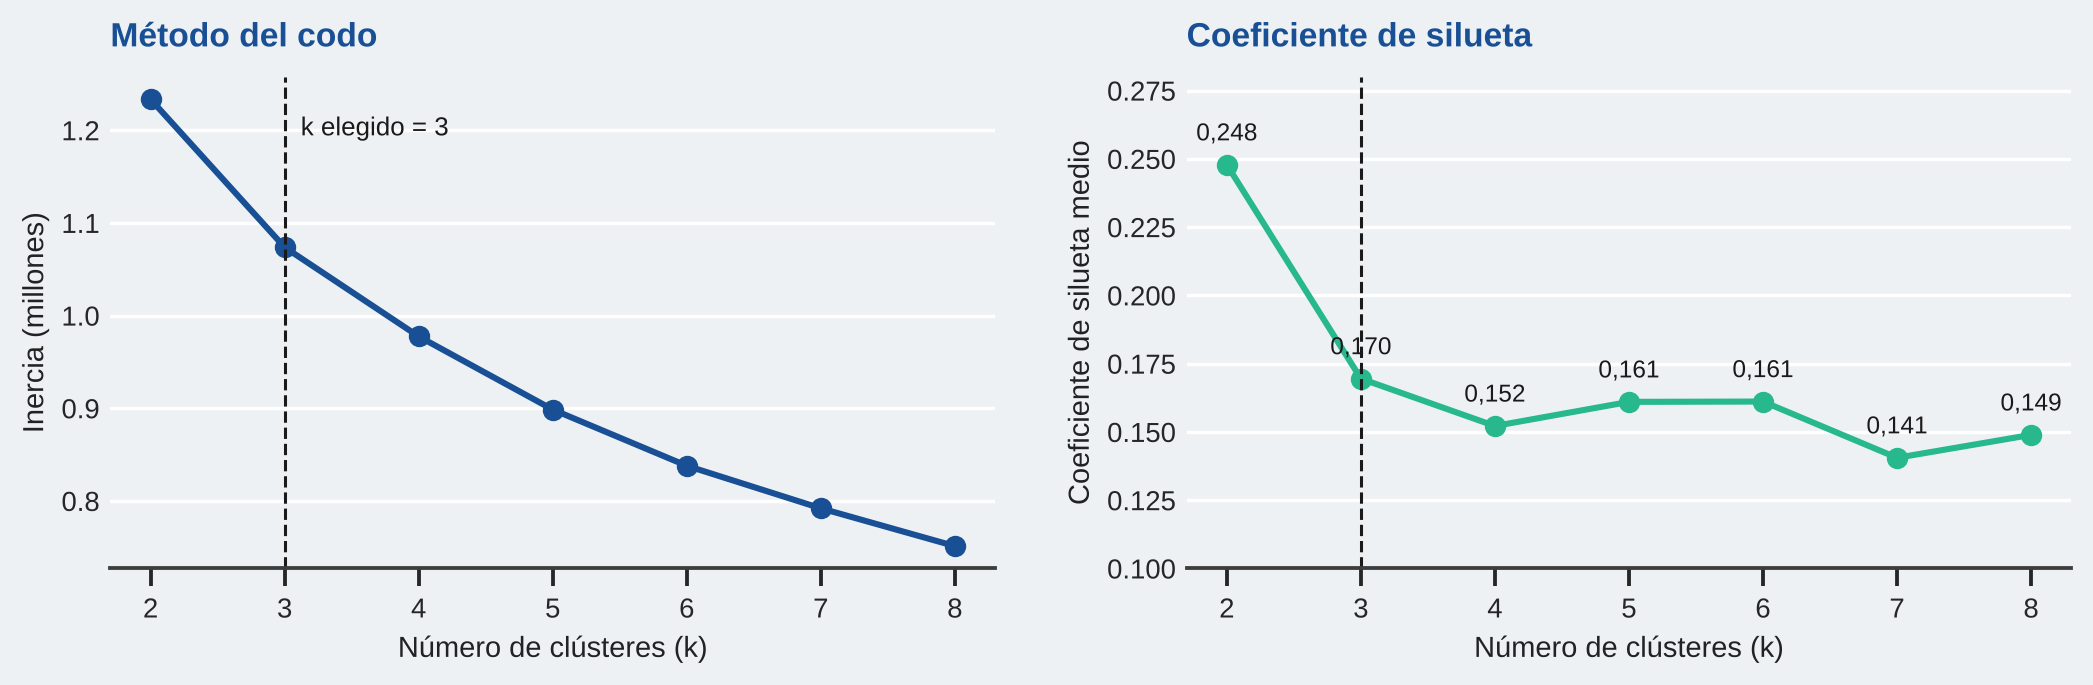
\includegraphics[width=\columnwidth]{figuras/fig2_codo_silueta.png}
\caption{Método del codo y coeficiente de silueta de K-Means.}
\label{fig:codo}
\end{figure}

\begin{table}[!t]
\centering
\caption{DBSCAN según $\varepsilon$ (\texttt{min\_samples}~$=16$)}
\label{tab:dbscan}
\scriptsize
\begin{tabular}{@{}rrrrr@{}}
\toprule
$\varepsilon$ & \textbf{Clúst.} & \textbf{Ruido (\%)} & \textbf{Mayor (\%)} & \textbf{Silueta} \\
\midrule
0{,}8 & 27 & 46{,}1 & 7{,}3 & 0{,}092 \\
1{,}0 & 5 & 34{,}6 & 29{,}1 & 0{,}070 \\
1{,}2 & 5 & 21{,}8 & 76{,}0 & 0{,}205 \\
1{,}5 & 4 & 7{,}9 & 88{,}4 & 0{,}253 \\
2{,}0 & 1 & 0{,}6 & 99{,}4 & -- \\
\bottomrule

\end{tabular}
\end{table}

\begin{table}[!t]
\centering
\caption{Perfil medio de los clústeres de K-Means}
\label{tab:perfiles}
\scriptsize
\begin{tabular}{@{}lrrr@{}}
\toprule
\textbf{Característica} & \textbf{C1} & \textbf{C2} & \textbf{C3} \\
\midrule
Población (\%) & 45{,}4 & 39{,}4 & 15{,}1 \\
Diabetes (\%) & 3{,}7 & 22{,}1 & 27{,}7 \\
IMC medio & 27{,}4 & 29{,}4 & 31{,}2 \\
Edad (código 1--13) & 5{,}9 & 10{,}2 & 8{,}3 \\
Salud general (1--5) & 2{,}0 & 2{,}7 & 3{,}9 \\
Días malestar físico & 1{,}3 & 1{,}6 & 21{,}1 \\
Días malestar mental & 3{,}4 & 1{,}3 & 14{,}3 \\
Hipertensión (\%) & 14{,}8 & 69{,}3 & 59{,}7 \\
Colesterol alto (\%) & 19{,}9 & 62{,}9 & 53{,}9 \\
Dificultad caminar (\%) & 2{,}1 & 16{,}9 & 51{,}0 \\
Ingreso (1--7) & 5{,}4 & 4{,}2 & 3{,}5 \\
\bottomrule

\end{tabular}
\end{table}

\begin{figure*}[!t]
\centering
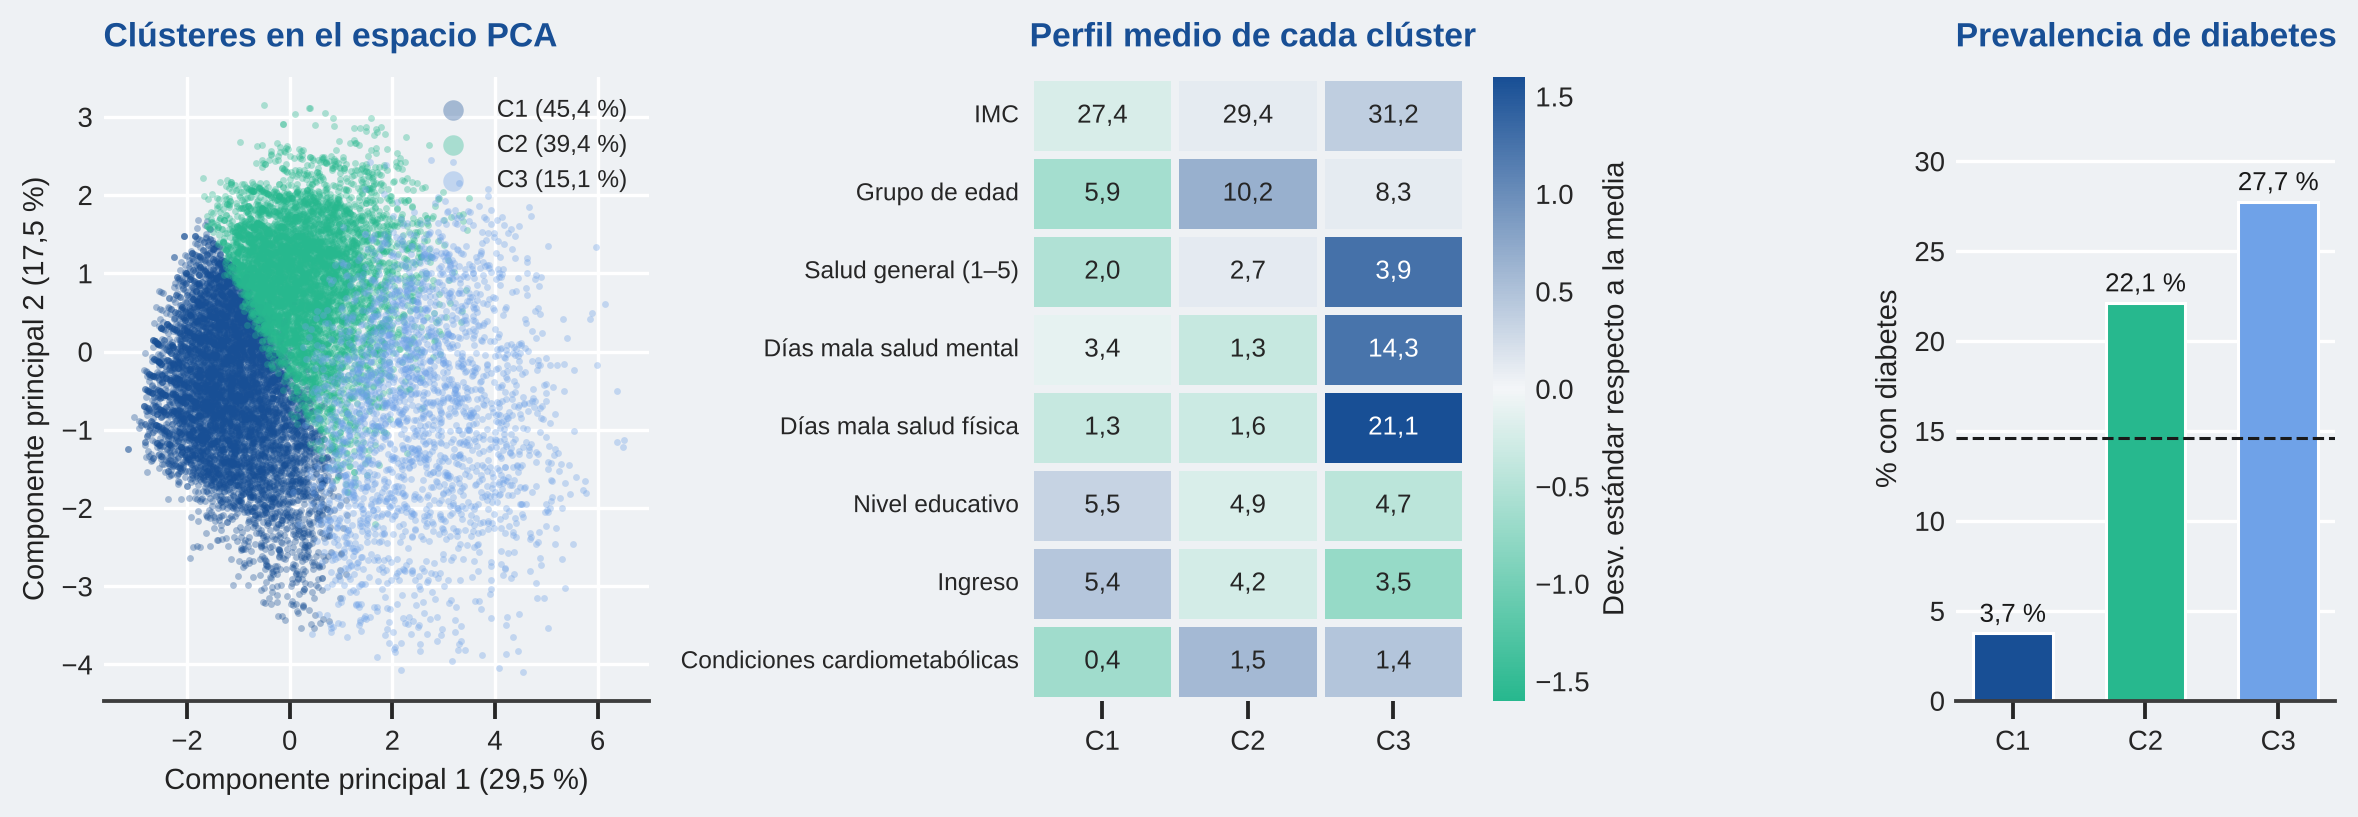
\includegraphics[width=0.92\textwidth]{figuras/fig3_clusters.png}
\caption{Clústeres en el espacio PCA, perfil medio estandarizado y prevalencia de diabetes por clúster.}
\label{fig:clusters}
\end{figure*}

\subsection{Interpretabilidad}\label{sec:shap}
Según TreeSHAP (Fig.~\ref{fig:shap}), las cinco variables principales concentran el 70\,\% del efecto: salud general percibida (0,492), interacción edad $\times$ IMC (0,485), CardioRisk (0,423), hipertensión (0,215) e IMC (0,202). Dos de las tres primeras son variables derivadas. La importancia por permutación coincide en las principales, lo que indica que el resultado no es un artefacto del método de explicación.

\begin{figure*}[!t]
\centering
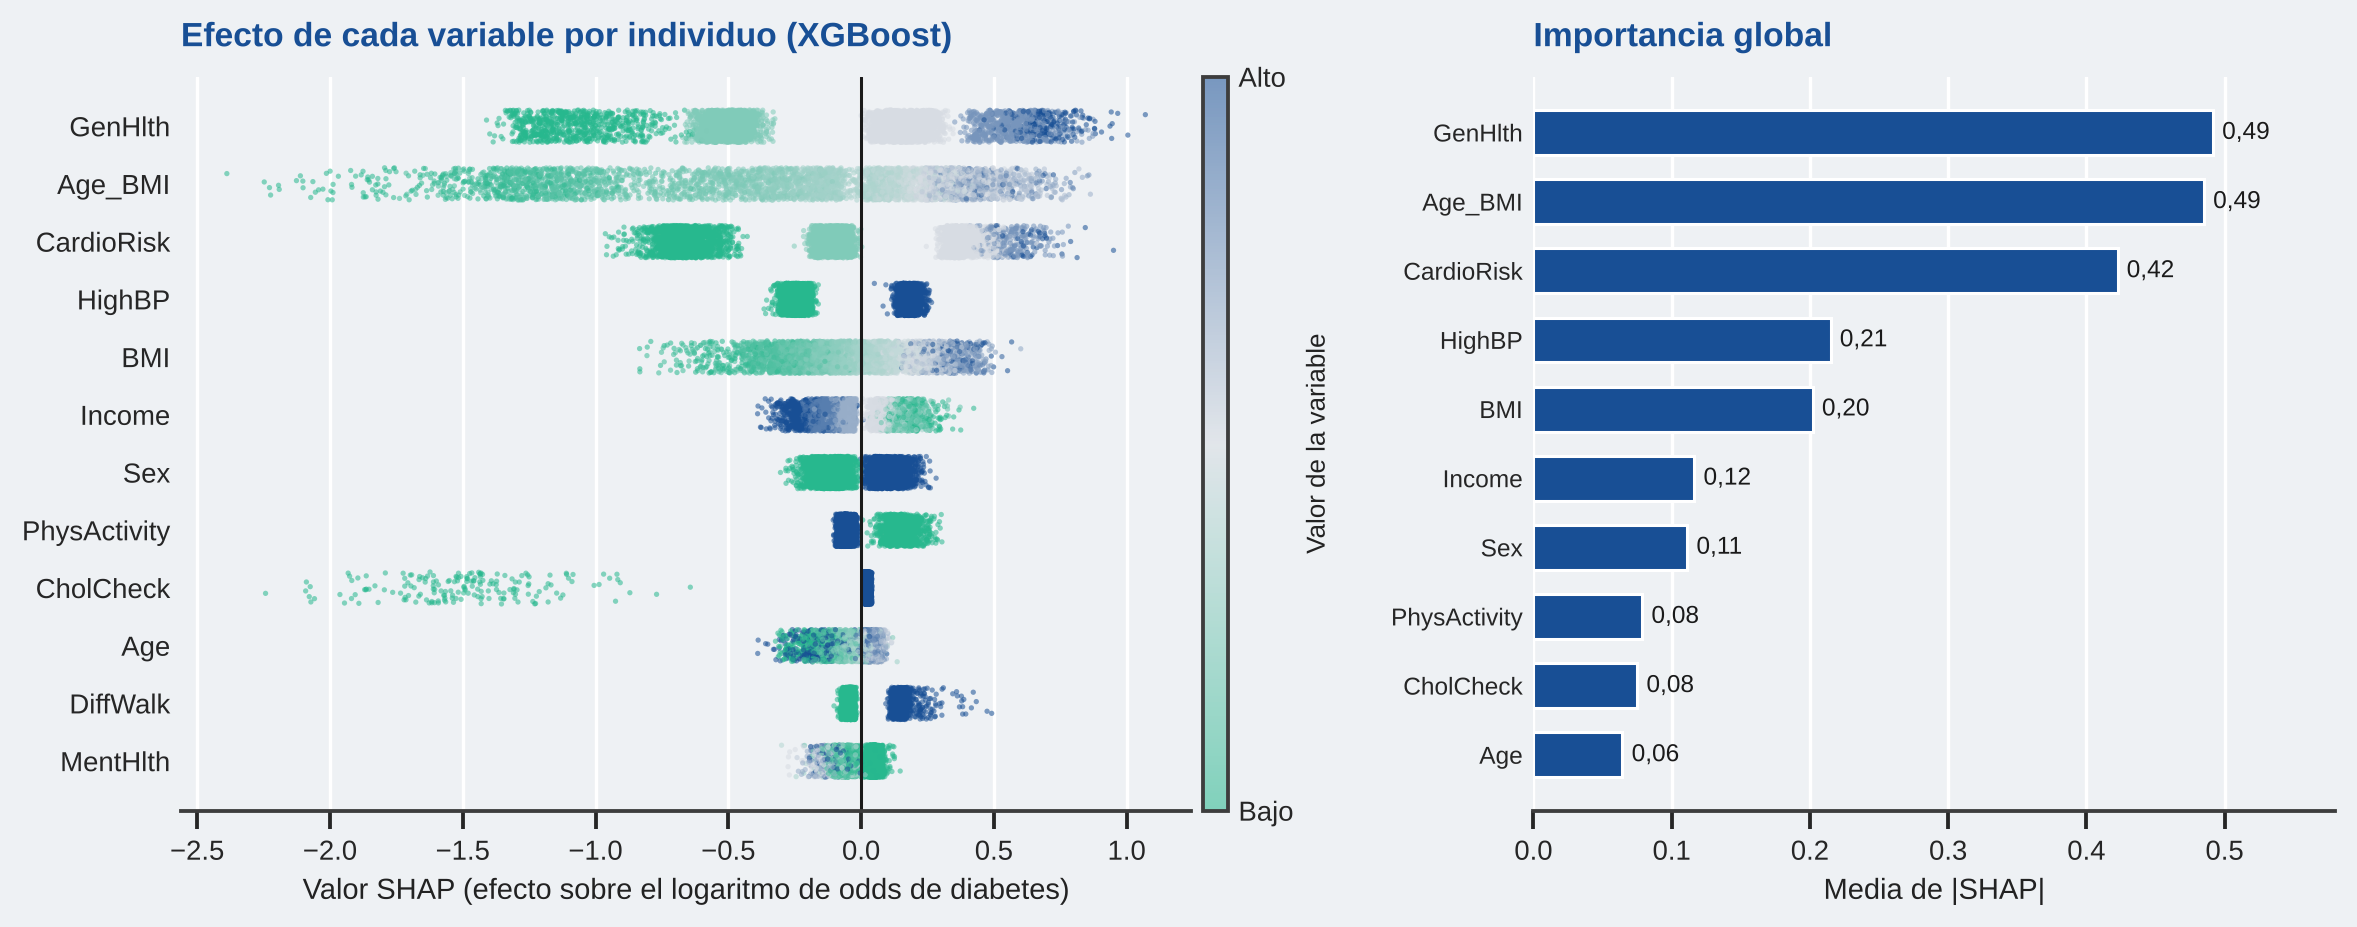
\includegraphics[width=0.8\textwidth]{figuras/fig7_shap.png}
\caption{Valores SHAP del modelo XGBoost: dirección de los efectos (izq.) e importancia global (der.).}
\label{fig:shap}
\end{figure*}

\subsection{Costo computacional y reproducibilidad}
El cuaderno de la Fase~3 se ejecuta en 8,0 minutos en una CPU de dos núcleos, sin GPU; la búsqueda de hiperparámetros ocupa 301~s. Reentrenar todos los modelos finales con el script del repositorio toma unos diez segundos y una predicción en la aplicación, milisegundos. La reejecución de los cuadernos en la estructura del repositorio reprodujo todos los valores de resultados, salvo los tiempos.

\subsection{Aplicación web desplegada}
La aplicación está desplegada en Streamlit Community Cloud y es de acceso público en \url{https://alainkapra-diabetes-brfss2023.streamlit.app}; se construye directamente desde la rama \texttt{main} del repositorio, de modo que cada cambio publicado se refleja en la versión en línea. La Fig.~\ref{fig:app} muestra tres módulos de la aplicación: las tarjetas KPI animadas del Panorama, la predicción en vivo con su cascada SHAP y la segmentación con la dispersión 3D en el espacio PCA, que puede girarse y colorearse por perfil o por diagnóstico.

\begin{figure*}[!t]
\centering
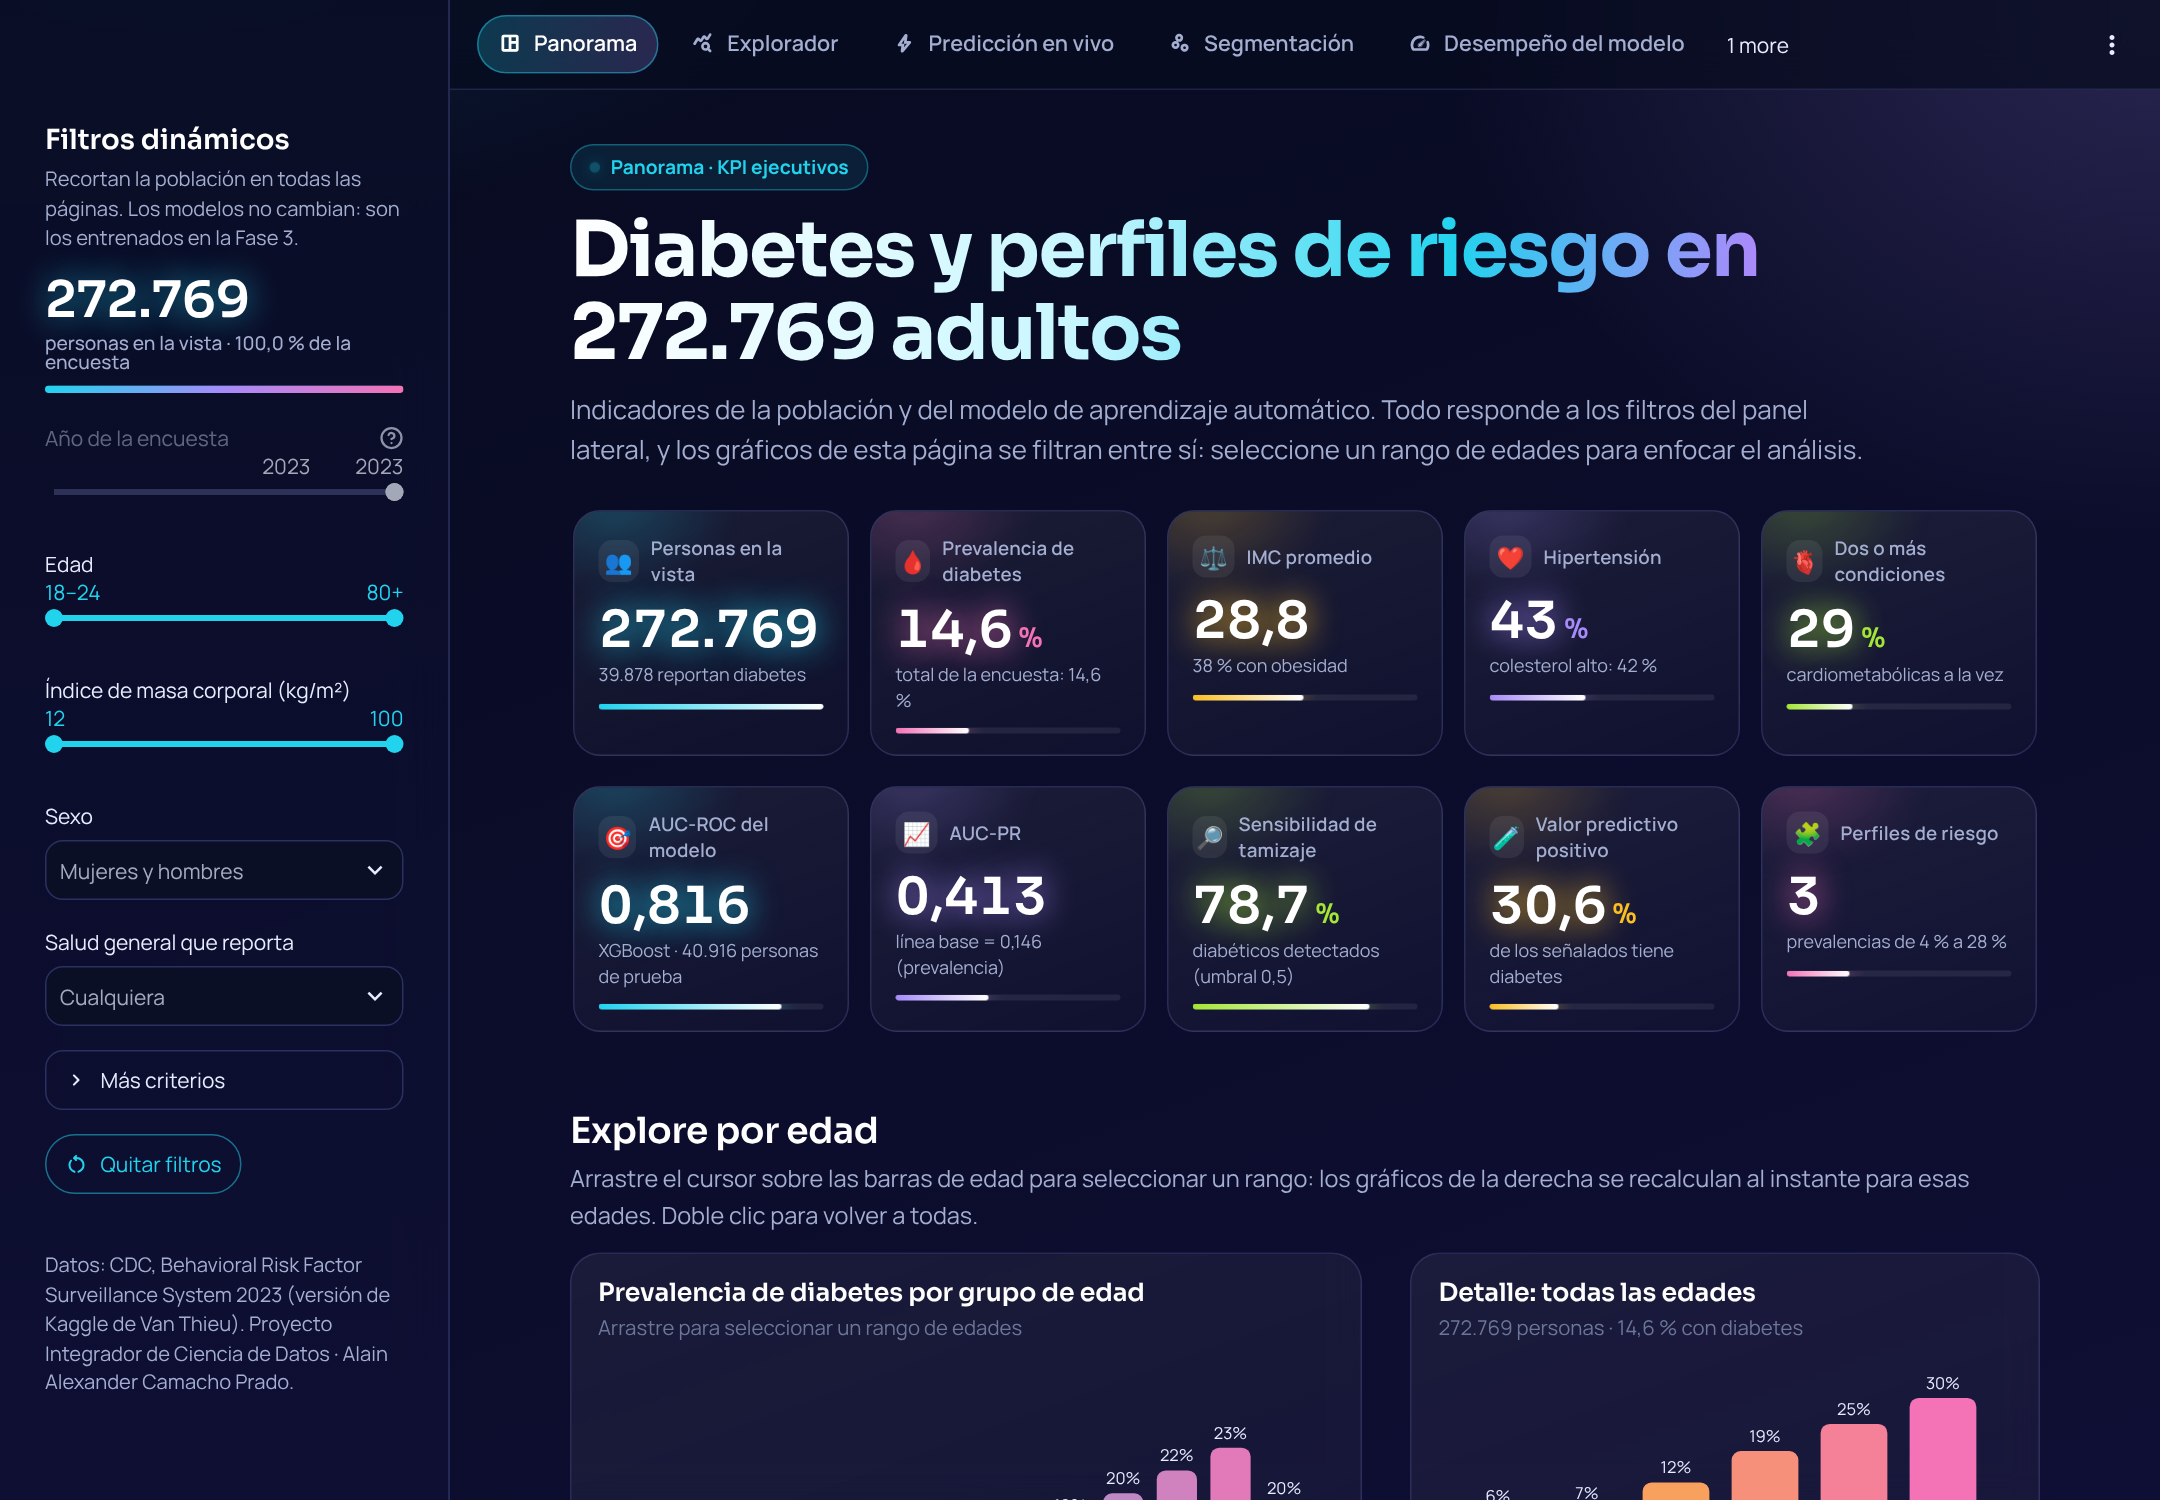
\includegraphics[width=0.325\textwidth]{figuras/dash1_panorama.png}\hfill
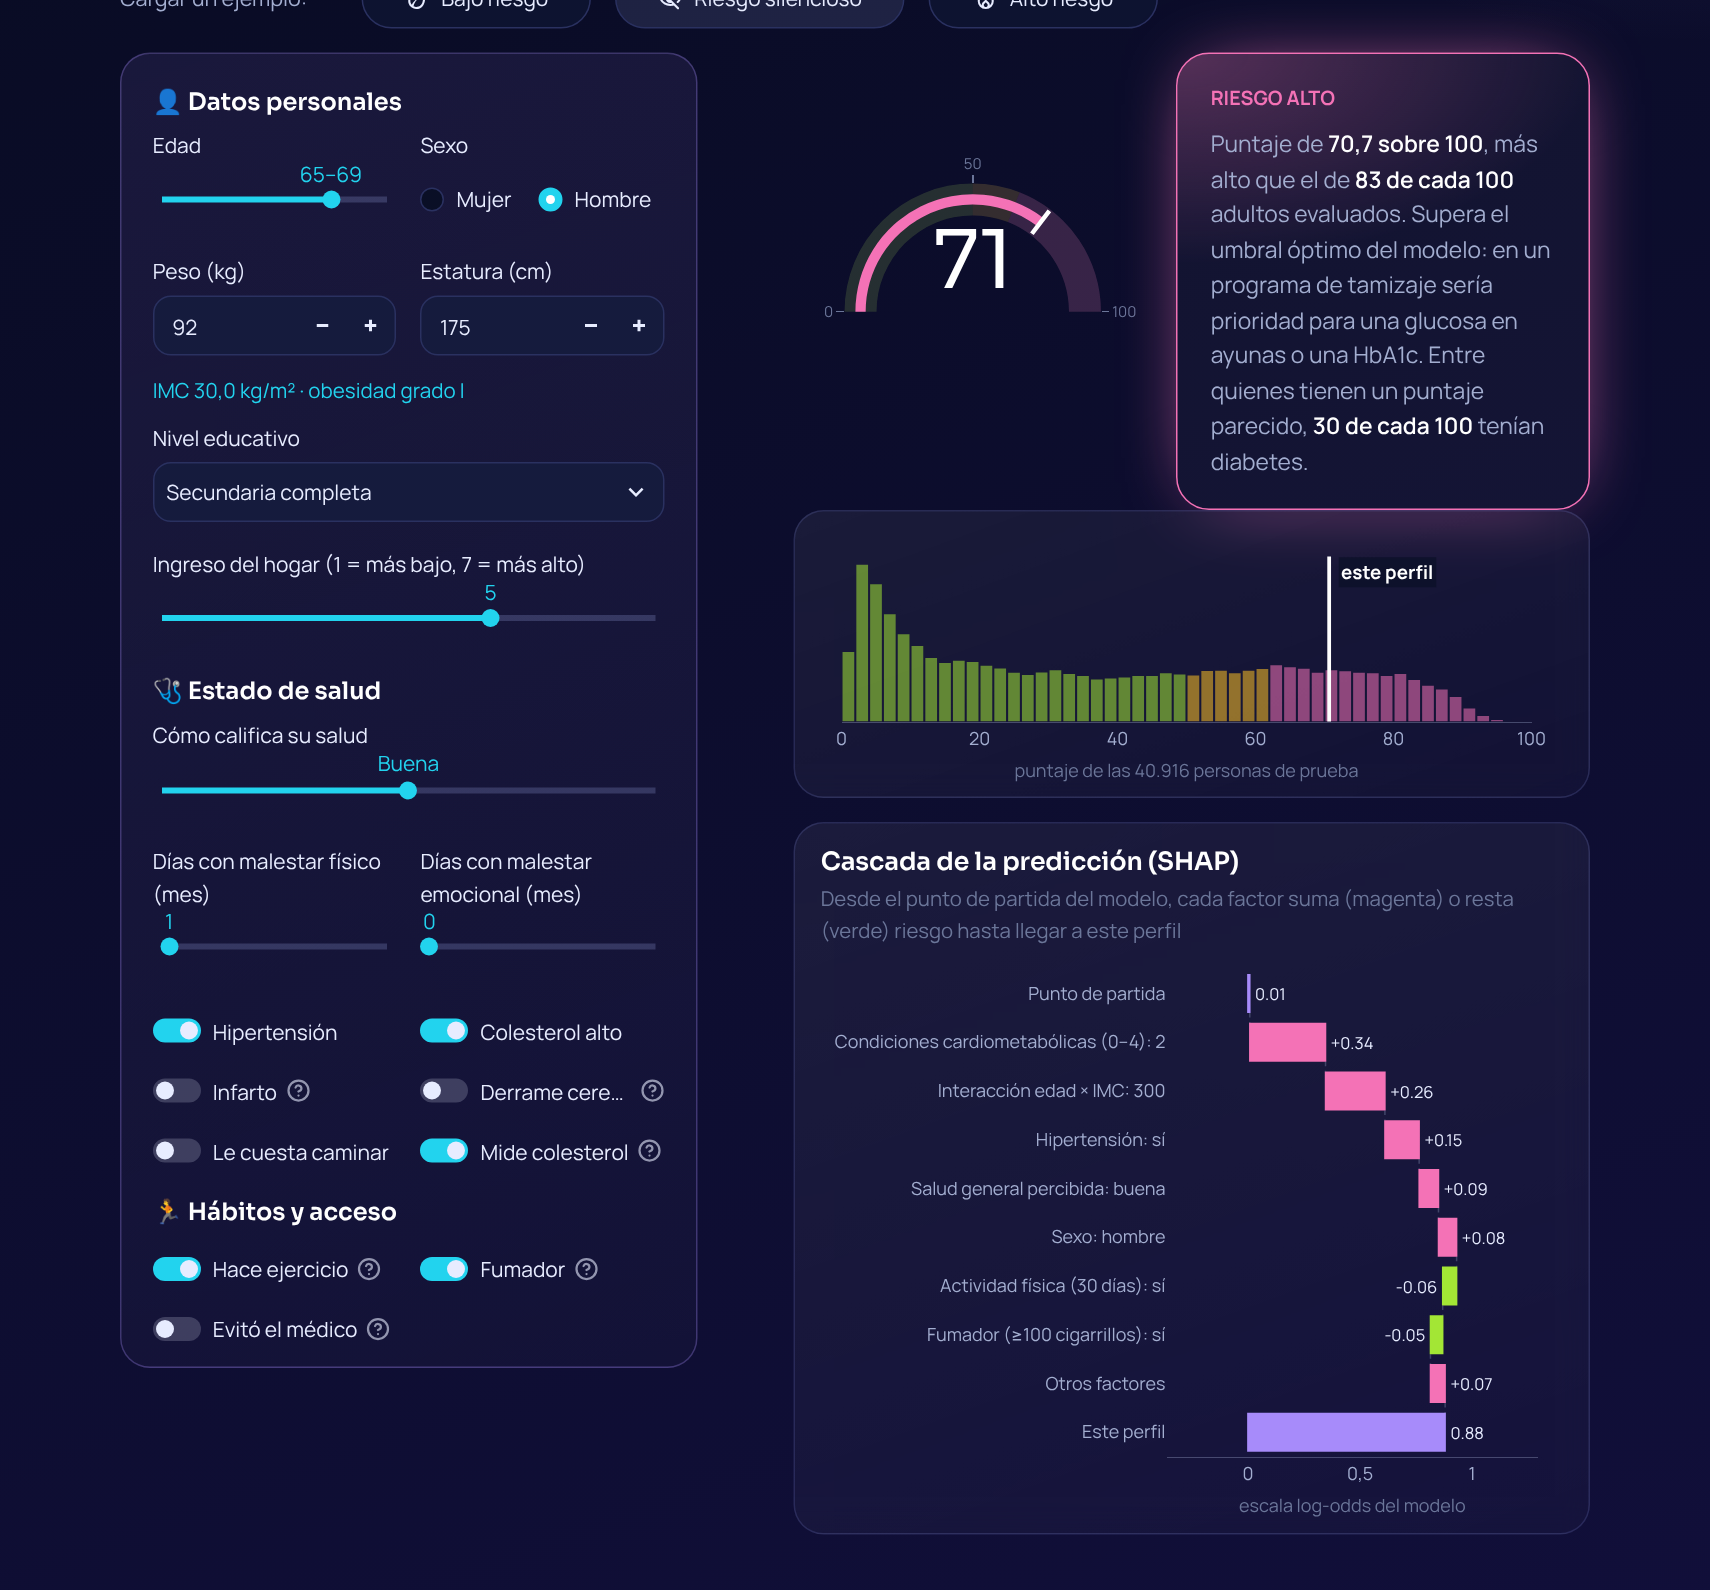
\includegraphics[width=0.325\textwidth]{figuras/dash3_prediccion.png}\hfill
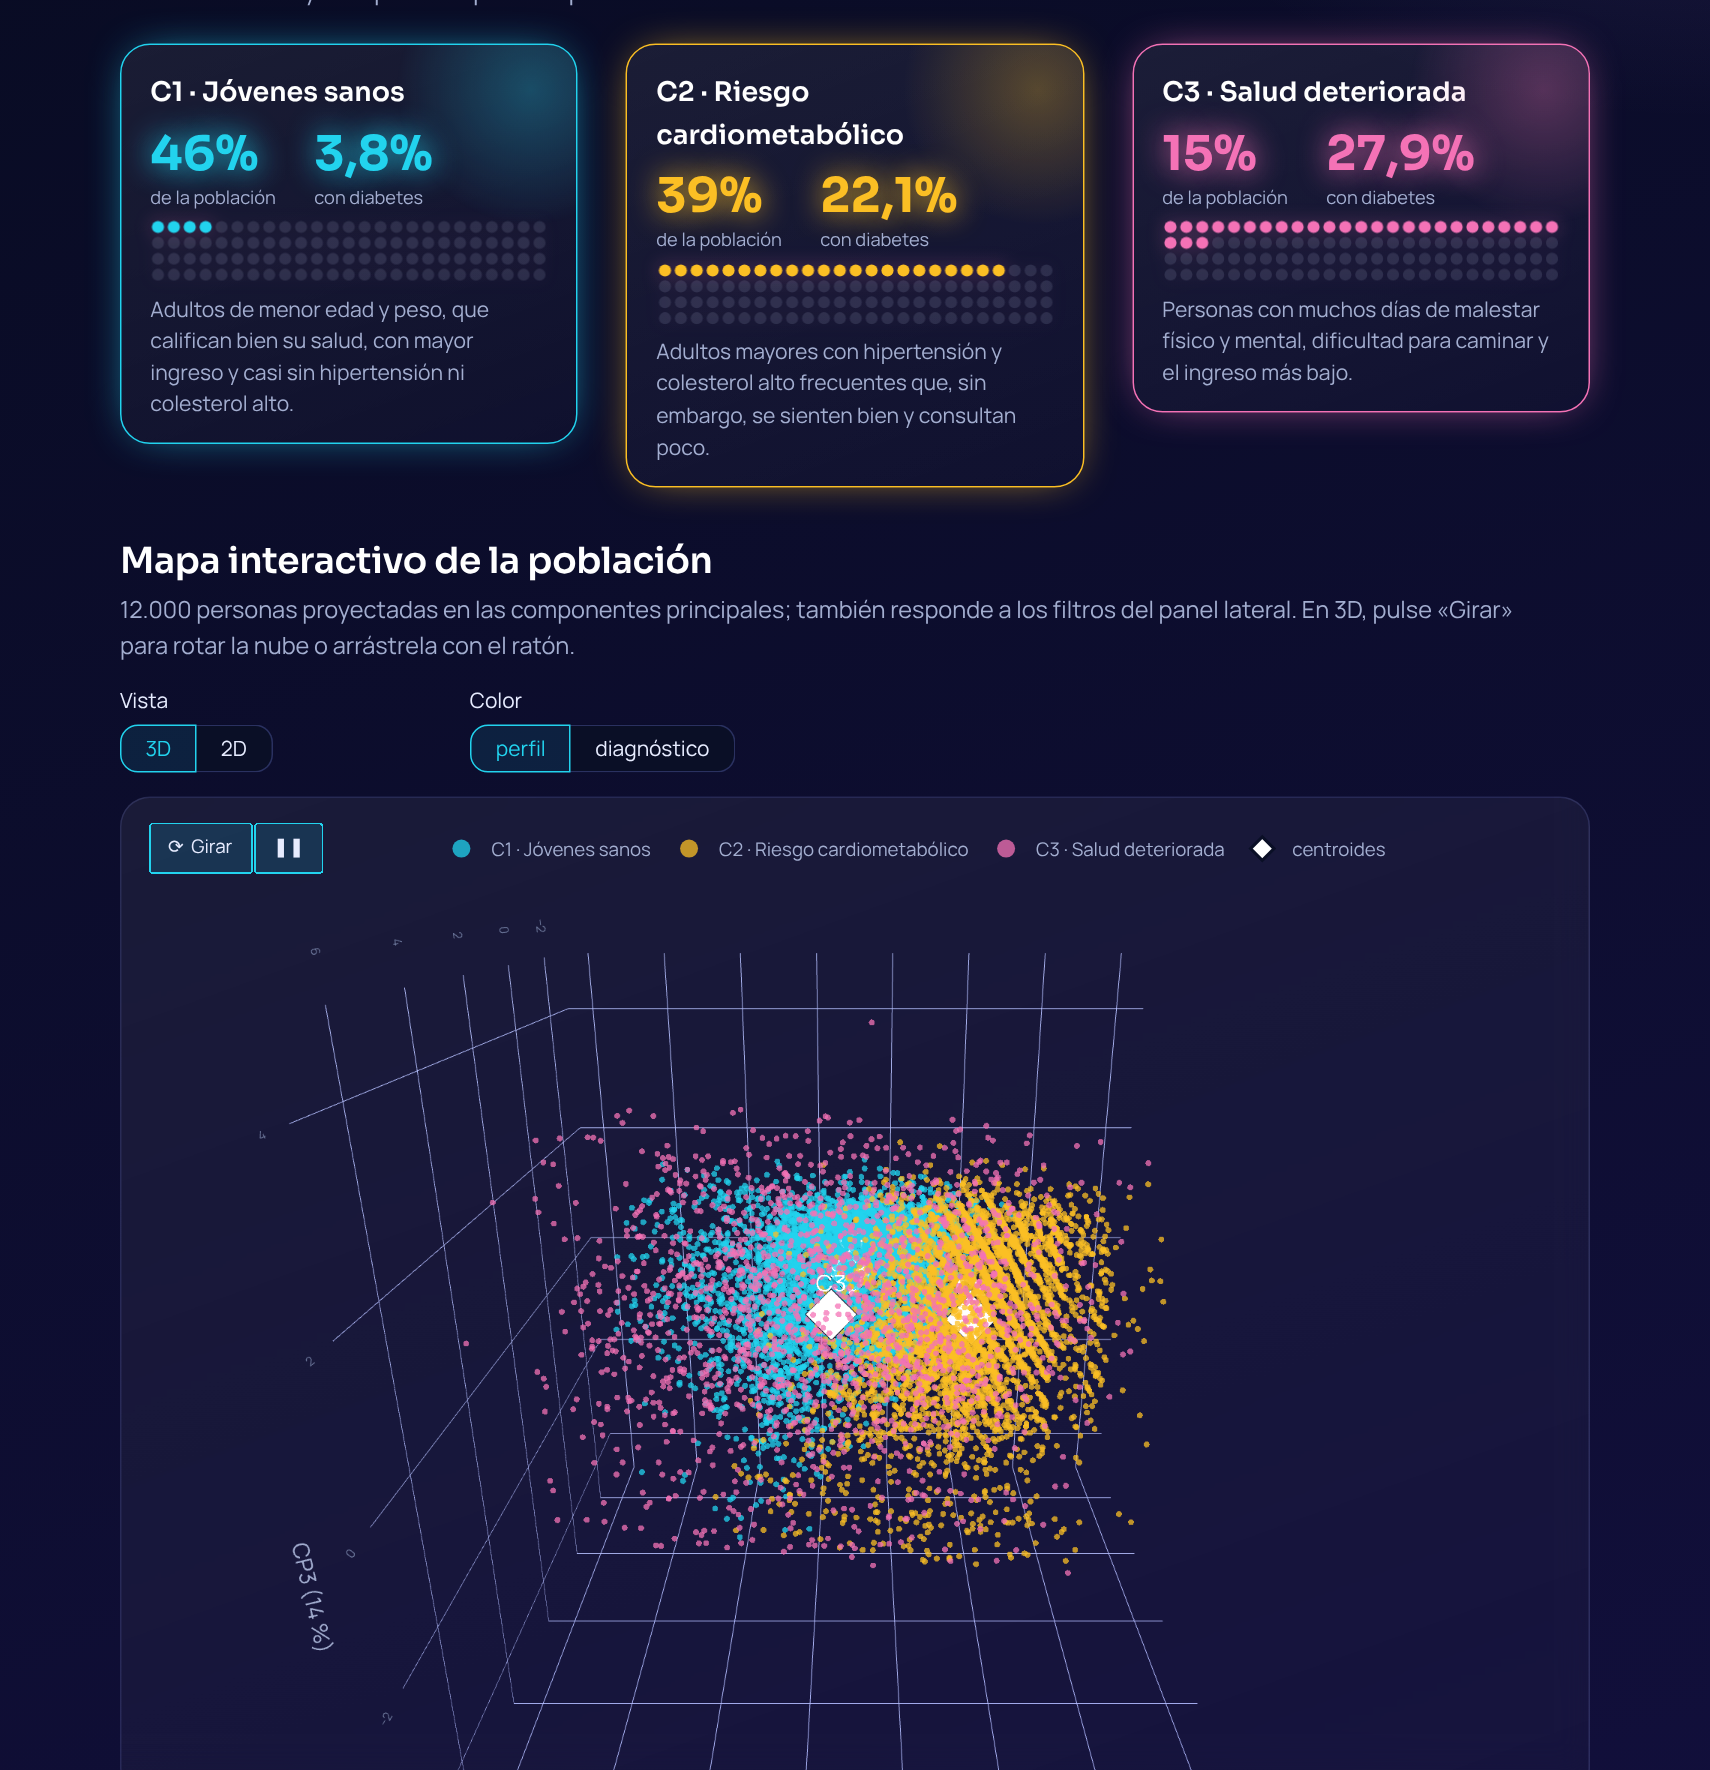
\includegraphics[width=0.325\textwidth]{figuras/dash4_segmentacion.png}
\caption{Aplicación web: (izq.) Panorama con filtros dinámicos y KPI; (centro) predicción en vivo con indicador, distribución y cascada SHAP; (der.) segmentación con perfiles y mapa 3D en el espacio PCA.}
\label{fig:app}
\end{figure*}

% =====================================================================
\section{Discusión}
% =====================================================================
\subsection{Un techo impuesto por los datos}
Modelos con sesgos inductivos muy distintos (lineal, \textit{bagging}, \textit{boosting} y red neuronal) convergen en AUC-ROC de 0,81--0,82, y la optimización no lo mueve. En la descomposición sesgo--varianza--ruido \cite{hastie2009}, esa convergencia indica que el error restante es en su mayoría irreducible con las variables disponibles. El resultado concuerda con estudios previos sobre la BRFSS ($\text{AUC}\approx 0{,}80$) \cite{xie2019}, mientras que modelos con variables de laboratorio logran valores mucho mayores \cite{dinh2019}. Por ello las metas de la Fase~1 (F1~$\geq0{,}70$; R$^2\geq0{,}25$) no se alcanzaron y se reformularon según el uso real del modelo, el tamizaje: AUC-ROC~$\geq0{,}80$ (logrado: 0,816), sensibilidad~$\geq0{,}75$ (0,787) y R$^2\geq0{,}18$ (0,186).

\subsection{Lecciones metodológicas}
\textbf{La fuga se previene por diseño.} Encapsular el preprocesamiento en \textit{pipelines} impidió por construcción que la validación cruzada viera datos de evaluación y permitió desplegar un único objeto que recibe datos crudos.

\textbf{Con desbalance, métrica y umbral son decisiones de diseño.} Un clasificador trivial logra 85\,\% de exactitud; el AUC-PR guió la selección y el umbral se trató como parámetro de la decisión (sensibilidad de 79\,\% o 64\,\% con el mismo modelo).

\textbf{En datos tabulares los árboles siguen siendo referencia.} La red neuronal necesitó escalamiento, codificación, pérdida ponderada y parada temprana para igualar a un XGBoost casi sin preprocesamiento.

\textbf{Los resultados nulos también informan.} Regularización, búsqueda de hiperparámetros y variables derivadas en el modelo lineal no mejoraron: documentarlo muestra dónde está el límite.

\textbf{El no supervisado exige criterio.} Con variables discretas la silueta es baja aunque los grupos tengan sentido; la validación externa y la concordancia entre algoritmos fueron más informativas que un índice aislado.

\textbf{Interpretabilidad y reproducibilidad son parte del producto.} SHAP confirmó relaciones coherentes y reveló un sesgo de detección (el control de colesterol se asocia con más diabetes porque quien consulta más recibe más diagnósticos).

\subsection{Interpretación aplicada}
La diabetes se acumula con hipertensión, colesterol alto y enfermedad cardiovascular; el peso actúa como una escalera y la edad amplifica su efecto. El perfil C2 (22,1\,\% con diabetes) se siente bien y consulta poco: es el principal destinatario de búsqueda activa. Con un valor predictivo positivo de 30,6\,\%, el modelo no diagnostica: ordena el riesgo para priorizar pruebas de laboratorio, y la aplicación hace visible ese compromiso, en línea con las recomendaciones de reporte transparente \cite{collins2015}.

\subsection{Limitaciones}
Los datos son autorreportados; el objetivo es la diabetes diagnosticada, de modo que los casos no diagnosticados figuran como negativos; el diseño es transversal; no se aplicaron pesos muestrales, y la población es estadounidense. En el modelado, los puntajes de XGBoost entrenado con pesos de clase no están calibrados \cite{vancalster2019} (la aplicación muestra una calibración empírica), la red neuronal no tuvo búsqueda de hiperparámetros propia, no se usó validación cruzada anidada y no se auditó la equidad por subgrupos.

% =====================================================================
\section{Conclusiones}
% =====================================================================
Se construyó, evaluó y desplegó una solución completa de ciencia de datos para el riesgo de diabetes. Un flujo sin fuga de datos, la comparación controlada de cuatro familias de clasificadores con validación cruzada, intervalos \textit{bootstrap} y un conjunto de prueba sellado condujo a un XGBoost con AUC-ROC de 0,816 y AUC-PR de 0,413 (2,8 veces la línea base). La convergencia de los modelos mostró que el límite está en la información disponible y no en el algoritmo, conclusión que solo el diseño experimental permite sostener. La segmentación identificó tres perfiles validados externamente y por un segundo algoritmo, y SHAP confirmó factores coherentes y en buena medida modificables. La aplicación web en Streamlit, con filtros dinámicos, KPI, predicción en vivo explicada y segmentación interactiva, junto con un repositorio con versiones exactas, código modular, pruebas y reentrenamiento reproducible, convierte el análisis en una herramienta verificable.

% =====================================================================
\section{Trabajo futuro}
% =====================================================================
\begin{itemize}
\item \textbf{Modelado:} optimización bayesiana con mayor presupuesto (incluida la red), LightGBM y CatBoost, restricciones de monotonía en XGBoost y validación cruzada anidada.
\item \textbf{Calibración y decisión:} regresión isotónica o de Platt y análisis de curvas de decisión para elegir el umbral según el costo de las pruebas.
\item \textbf{Equidad y validez externa:} auditoría por sexo, edad e ingreso; validación temporal con los ciclos 2015--2022 de la BRFSS y adaptación con datos colombianos.
\item \textbf{Datos:} variables de laboratorio (glucosa, HbA1c), perímetro de cintura y antecedentes familiares; uso de pesos muestrales.
\item \textbf{MLOps:} registro de experimentos con MLflow, contenedores, integración continua y monitoreo de deriva en producción.
\end{itemize}

\section*{Disponibilidad de código y datos}
Repositorio público: \url{https://github.com/alainkapra/proyecto-diabetes-brfss2023} (estructura \texttt{/data}, \texttt{/notebooks}, \texttt{/src}, \texttt{/dashboard}; \texttt{requirements.txt} y \texttt{environment.yml} con versiones exactas). Aplicación desplegada: \url{https://alainkapra-diabetes-brfss2023.streamlit.app}.

\bibliographystyle{IEEEtran}
\bibliography{referencias}

\end{document}
